\documentclass[twoside]{book}

% Packages required by doxygen
\usepackage{fixltx2e}
\usepackage{calc}
\usepackage{doxygen}
\usepackage[export]{adjustbox} % also loads graphicx
\usepackage{graphicx}
\usepackage[utf8]{inputenc}
\usepackage{makeidx}
\usepackage{multicol}
\usepackage{multirow}
\PassOptionsToPackage{warn}{textcomp}
\usepackage{textcomp}
\usepackage[nointegrals]{wasysym}
\usepackage[table]{xcolor}

% Font selection
\usepackage[T1]{fontenc}
\usepackage[scaled=.90]{helvet}
\usepackage{courier}
\usepackage{amssymb}
\usepackage{sectsty}
\renewcommand{\familydefault}{\sfdefault}
\allsectionsfont{%
  \fontseries{bc}\selectfont%
  \color{darkgray}%
}
\renewcommand{\DoxyLabelFont}{%
  \fontseries{bc}\selectfont%
  \color{darkgray}%
}
\newcommand{\+}{\discretionary{\mbox{\scriptsize$\hookleftarrow$}}{}{}}

% Page & text layout
\usepackage{geometry}
\geometry{%
  a4paper,%
  top=2.5cm,%
  bottom=2.5cm,%
  left=2.5cm,%
  right=2.5cm%
}
\tolerance=750
\hfuzz=15pt
\hbadness=750
\setlength{\emergencystretch}{15pt}
\setlength{\parindent}{0cm}
\setlength{\parskip}{3ex plus 2ex minus 2ex}
\makeatletter
\renewcommand{\paragraph}{%
  \@startsection{paragraph}{4}{0ex}{-1.0ex}{1.0ex}{%
    \normalfont\normalsize\bfseries\SS@parafont%
  }%
}
\renewcommand{\subparagraph}{%
  \@startsection{subparagraph}{5}{0ex}{-1.0ex}{1.0ex}{%
    \normalfont\normalsize\bfseries\SS@subparafont%
  }%
}
\makeatother

% Headers & footers
\usepackage{fancyhdr}
\pagestyle{fancyplain}
\fancyhead[LE]{\fancyplain{}{\bfseries\thepage}}
\fancyhead[CE]{\fancyplain{}{}}
\fancyhead[RE]{\fancyplain{}{\bfseries\leftmark}}
\fancyhead[LO]{\fancyplain{}{\bfseries\rightmark}}
\fancyhead[CO]{\fancyplain{}{}}
\fancyhead[RO]{\fancyplain{}{\bfseries\thepage}}
\fancyfoot[LE]{\fancyplain{}{}}
\fancyfoot[CE]{\fancyplain{}{}}
\fancyfoot[RE]{\fancyplain{}{\bfseries\scriptsize Generated by Doxygen }}
\fancyfoot[LO]{\fancyplain{}{\bfseries\scriptsize Generated by Doxygen }}
\fancyfoot[CO]{\fancyplain{}{}}
\fancyfoot[RO]{\fancyplain{}{}}
\renewcommand{\footrulewidth}{0.4pt}
\renewcommand{\chaptermark}[1]{%
  \markboth{#1}{}%
}
\renewcommand{\sectionmark}[1]{%
  \markright{\thesection\ #1}%
}

% Indices & bibliography
\usepackage{natbib}
\usepackage[titles]{tocloft}
\setcounter{tocdepth}{3}
\setcounter{secnumdepth}{5}
\makeindex

% Hyperlinks (required, but should be loaded last)
\usepackage{ifpdf}
\ifpdf
  \usepackage[pdftex,pagebackref=true]{hyperref}
\else
  \usepackage[ps2pdf,pagebackref=true]{hyperref}
\fi
\hypersetup{%
  colorlinks=true,%
  linkcolor=blue,%
  citecolor=blue,%
  unicode%
}

% Custom commands
\newcommand{\clearemptydoublepage}{%
  \newpage{\pagestyle{empty}\cleardoublepage}%
}

\usepackage{caption}
\captionsetup{labelsep=space,justification=centering,font={bf},singlelinecheck=off,skip=4pt,position=top}

%===== C O N T E N T S =====

\begin{document}

% Titlepage & ToC
\hypersetup{pageanchor=false,
             bookmarksnumbered=true,
             pdfencoding=unicode
            }
\pagenumbering{alph}
\begin{titlepage}
\vspace*{7cm}
\begin{center}%
{\Large O\+G\+L\+\_\+\+Scene\+Loader }\\
\vspace*{1cm}
{\large Generated by Doxygen 1.8.14}\\
\end{center}
\end{titlepage}
\clearemptydoublepage
\pagenumbering{roman}
\tableofcontents
\clearemptydoublepage
\pagenumbering{arabic}
\hypersetup{pageanchor=true}

%--- Begin generated contents ---
\chapter{Namespace Index}
\section{Namespace List}
Here is a list of all namespaces with brief descriptions\+:\begin{DoxyCompactList}
\item\contentsline{section}{\mbox{\hyperlink{namespaceexample}{example}} }{\pageref{namespaceexample}}{}
\item\contentsline{section}{\mbox{\hyperlink{namespaceoglsl}{oglsl}} }{\pageref{namespaceoglsl}}{}
\end{DoxyCompactList}

\chapter{Hierarchical Index}
\section{Class Hierarchy}
This inheritance list is sorted roughly, but not completely, alphabetically\+:\begin{DoxyCompactList}
\item \contentsline{section}{oglsl\+:\+:Camera}{\pageref{classoglsl_1_1_camera}}{}
\item \contentsline{section}{oglsl\+:\+:Color\+\_\+\+Buffer\+\_\+\+Rgba8888\+:\+:Color}{\pageref{structoglsl_1_1_color___buffer___rgba8888_1_1_color}}{}
\item \contentsline{section}{oglsl\+:\+:Color\+\_\+\+Buffer}{\pageref{classoglsl_1_1_color___buffer}}{}
\begin{DoxyCompactList}
\item \contentsline{section}{oglsl\+:\+:Color\+\_\+\+Buffer\+\_\+\+Rgba8888}{\pageref{classoglsl_1_1_color___buffer___rgba8888}}{}
\end{DoxyCompactList}
\item \contentsline{section}{oglsl\+:\+:Cube}{\pageref{classoglsl_1_1_cube}}{}
\item \contentsline{section}{oglsl\+:\+:Framebuffer}{\pageref{classoglsl_1_1_framebuffer}}{}
\item \contentsline{section}{oglsl\+:\+:Input}{\pageref{classoglsl_1_1_input}}{}
\item \contentsline{section}{oglsl\+:\+:Mesh}{\pageref{classoglsl_1_1_mesh}}{}
\item \contentsline{section}{oglsl\+:\+:Node}{\pageref{classoglsl_1_1_node}}{}
\begin{DoxyCompactList}
\item \contentsline{section}{oglsl\+:\+:Elevation\+\_\+\+Mesh}{\pageref{classoglsl_1_1_elevation___mesh}}{}
\item \contentsline{section}{oglsl\+:\+:Model}{\pageref{classoglsl_1_1_model}}{}
\end{DoxyCompactList}
\item \contentsline{section}{oglsl\+:\+:Scene}{\pageref{classoglsl_1_1_scene}}{}
\begin{DoxyCompactList}
\item \contentsline{section}{oglsl\+:\+:my\+Scene}{\pageref{classoglsl_1_1my_scene}}{}
\end{DoxyCompactList}
\item \contentsline{section}{oglsl\+:\+:Shader}{\pageref{classoglsl_1_1_shader}}{}
\begin{DoxyCompactList}
\item \contentsline{section}{oglsl\+:\+:Fragment\+\_\+\+Shader}{\pageref{classoglsl_1_1_fragment___shader}}{}
\item \contentsline{section}{oglsl\+:\+:Vertex\+\_\+\+Shader}{\pageref{classoglsl_1_1_vertex___shader}}{}
\end{DoxyCompactList}
\item \contentsline{section}{oglsl\+:\+:Shader\+\_\+\+Program}{\pageref{classoglsl_1_1_shader___program}}{}
\item \contentsline{section}{oglsl\+:\+:Skybox}{\pageref{classoglsl_1_1_skybox}}{}
\item \contentsline{section}{oglsl\+:\+:Shader\+:\+:Source\+\_\+\+Code}{\pageref{classoglsl_1_1_shader_1_1_source___code}}{}
\item \contentsline{section}{oglsl\+:\+:Texture\+\_\+\+Cube}{\pageref{classoglsl_1_1_texture___cube}}{}
\item \contentsline{section}{oglsl\+:\+:Variant}{\pageref{classoglsl_1_1_variant}}{}
\item \contentsline{section}{oglsl\+:\+:View}{\pageref{classoglsl_1_1_view}}{}
\end{DoxyCompactList}

\chapter{Class Index}
\section{Class List}
Here are the classes, structs, unions and interfaces with brief descriptions\+:\begin{DoxyCompactList}
\item\contentsline{section}{\mbox{\hyperlink{structexample_1_1_color___buffer___rgba8888_1_1_color}{example\+::\+Color\+\_\+\+Buffer\+\_\+\+Rgba8888\+::\+Color}} }{\pageref{structexample_1_1_color___buffer___rgba8888_1_1_color}}{}
\item\contentsline{section}{\mbox{\hyperlink{classexample_1_1_color___buffer}{example\+::\+Color\+\_\+\+Buffer}} }{\pageref{classexample_1_1_color___buffer}}{}
\item\contentsline{section}{\mbox{\hyperlink{classexample_1_1_color___buffer___rgba8888}{example\+::\+Color\+\_\+\+Buffer\+\_\+\+Rgba8888}} }{\pageref{classexample_1_1_color___buffer___rgba8888}}{}
\item\contentsline{section}{\mbox{\hyperlink{classexample_1_1_cube}{example\+::\+Cube}} }{\pageref{classexample_1_1_cube}}{}
\item\contentsline{section}{\mbox{\hyperlink{classexample_1_1_elevation___mesh}{example\+::\+Elevation\+\_\+\+Mesh}} }{\pageref{classexample_1_1_elevation___mesh}}{}
\item\contentsline{section}{\mbox{\hyperlink{classexample_1_1_input}{example\+::\+Input}} }{\pageref{classexample_1_1_input}}{}
\item\contentsline{section}{\mbox{\hyperlink{classexample_1_1_mesh}{example\+::\+Mesh}} }{\pageref{classexample_1_1_mesh}}{}
\item\contentsline{section}{\mbox{\hyperlink{classexample_1_1_model}{example\+::\+Model}} }{\pageref{classexample_1_1_model}}{}
\item\contentsline{section}{\mbox{\hyperlink{classexample_1_1_node}{example\+::\+Node}} }{\pageref{classexample_1_1_node}}{}
\item\contentsline{section}{\mbox{\hyperlink{classexample_1_1_scene}{example\+::\+Scene}} }{\pageref{classexample_1_1_scene}}{}
\item\contentsline{section}{\mbox{\hyperlink{classexample_1_1_view}{example\+::\+View}} }{\pageref{classexample_1_1_view}}{}
\end{DoxyCompactList}

\chapter{File Index}
\section{File List}
Here is a list of all files with brief descriptions\+:\begin{DoxyCompactList}
\item\contentsline{section}{D\+:/\+Git\+Kraken/3\+D\+Av\+\_\+2/src/\mbox{\hyperlink{_color___buffer_8hpp}{Color\+\_\+\+Buffer.\+hpp}} }{\pageref{_color___buffer_8hpp}}{}
\item\contentsline{section}{D\+:/\+Git\+Kraken/3\+D\+Av\+\_\+2/src/\mbox{\hyperlink{_color___buffer___rgba8888_8hpp}{Color\+\_\+\+Buffer\+\_\+\+Rgba8888.\+hpp}} }{\pageref{_color___buffer___rgba8888_8hpp}}{}
\item\contentsline{section}{D\+:/\+Git\+Kraken/3\+D\+Av\+\_\+2/src/\mbox{\hyperlink{_cube_8cpp}{Cube.\+cpp}} }{\pageref{_cube_8cpp}}{}
\item\contentsline{section}{D\+:/\+Git\+Kraken/3\+D\+Av\+\_\+2/src/\mbox{\hyperlink{_cube_8hpp}{Cube.\+hpp}} }{\pageref{_cube_8hpp}}{}
\item\contentsline{section}{D\+:/\+Git\+Kraken/3\+D\+Av\+\_\+2/src/\mbox{\hyperlink{_elevation___mesh_8cpp}{Elevation\+\_\+\+Mesh.\+cpp}} }{\pageref{_elevation___mesh_8cpp}}{}
\item\contentsline{section}{D\+:/\+Git\+Kraken/3\+D\+Av\+\_\+2/src/\mbox{\hyperlink{_elevation___mesh_8hpp}{Elevation\+\_\+\+Mesh.\+hpp}} }{\pageref{_elevation___mesh_8hpp}}{}
\item\contentsline{section}{D\+:/\+Git\+Kraken/3\+D\+Av\+\_\+2/src/\mbox{\hyperlink{_input_8hpp}{Input.\+hpp}} }{\pageref{_input_8hpp}}{}
\item\contentsline{section}{D\+:/\+Git\+Kraken/3\+D\+Av\+\_\+2/src/\mbox{\hyperlink{main_8cpp}{main.\+cpp}} }{\pageref{main_8cpp}}{}
\item\contentsline{section}{D\+:/\+Git\+Kraken/3\+D\+Av\+\_\+2/src/\mbox{\hyperlink{_mesh_8cpp}{Mesh.\+cpp}} }{\pageref{_mesh_8cpp}}{}
\item\contentsline{section}{D\+:/\+Git\+Kraken/3\+D\+Av\+\_\+2/src/\mbox{\hyperlink{_mesh_8hpp}{Mesh.\+hpp}} }{\pageref{_mesh_8hpp}}{}
\item\contentsline{section}{D\+:/\+Git\+Kraken/3\+D\+Av\+\_\+2/src/\mbox{\hyperlink{_model_8cpp}{Model.\+cpp}} }{\pageref{_model_8cpp}}{}
\item\contentsline{section}{D\+:/\+Git\+Kraken/3\+D\+Av\+\_\+2/src/\mbox{\hyperlink{_model_8hpp}{Model.\+hpp}} }{\pageref{_model_8hpp}}{}
\item\contentsline{section}{D\+:/\+Git\+Kraken/3\+D\+Av\+\_\+2/src/\mbox{\hyperlink{_node_8hpp}{Node.\+hpp}} }{\pageref{_node_8hpp}}{}
\item\contentsline{section}{D\+:/\+Git\+Kraken/3\+D\+Av\+\_\+2/src/\mbox{\hyperlink{_scene_8hpp}{Scene.\+hpp}} }{\pageref{_scene_8hpp}}{}
\item\contentsline{section}{D\+:/\+Git\+Kraken/3\+D\+Av\+\_\+2/src/\mbox{\hyperlink{_view_8cpp}{View.\+cpp}} }{\pageref{_view_8cpp}}{}
\item\contentsline{section}{D\+:/\+Git\+Kraken/3\+D\+Av\+\_\+2/src/\mbox{\hyperlink{_view_8hpp}{View.\+hpp}} }{\pageref{_view_8hpp}}{}
\end{DoxyCompactList}

\chapter{Namespace Documentation}
\hypertarget{namespaceexample}{}\section{example Namespace Reference}
\label{namespaceexample}\index{example@{example}}
\subsection*{Classes}
\begin{DoxyCompactItemize}
\item 
class \mbox{\hyperlink{classexample_1_1_color___buffer}{Color\+\_\+\+Buffer}}
\item 
class \mbox{\hyperlink{classexample_1_1_color___buffer___rgba8888}{Color\+\_\+\+Buffer\+\_\+\+Rgba8888}}
\item 
class \mbox{\hyperlink{classexample_1_1_cube}{Cube}}
\item 
class \mbox{\hyperlink{classexample_1_1_elevation___mesh}{Elevation\+\_\+\+Mesh}}
\item 
class \mbox{\hyperlink{classexample_1_1_input}{Input}}
\item 
class \mbox{\hyperlink{classexample_1_1_mesh}{Mesh}}
\item 
class \mbox{\hyperlink{classexample_1_1_model}{Model}}
\item 
class \mbox{\hyperlink{classexample_1_1_node}{Node}}
\item 
class \mbox{\hyperlink{classexample_1_1_scene}{Scene}}
\item 
class \mbox{\hyperlink{classexample_1_1_view}{View}}
\end{DoxyCompactItemize}
\subsection*{Typedefs}
\begin{DoxyCompactItemize}
\item 
typedef \mbox{\hyperlink{classexample_1_1_color___buffer___rgba8888}{Color\+\_\+\+Buffer\+\_\+\+Rgba8888}} \mbox{\hyperlink{namespaceexample_a4e4424d0fb5b457e8c00b8a7cdaad0e6}{Texture}}
\end{DoxyCompactItemize}


\subsection{Typedef Documentation}
\mbox{\Hypertarget{namespaceexample_a4e4424d0fb5b457e8c00b8a7cdaad0e6}\label{namespaceexample_a4e4424d0fb5b457e8c00b8a7cdaad0e6}} 
\index{example@{example}!Texture@{Texture}}
\index{Texture@{Texture}!example@{example}}
\subsubsection{\texorpdfstring{Texture}{Texture}}
{\footnotesize\ttfamily typedef \mbox{\hyperlink{classexample_1_1_color___buffer___rgba8888}{Color\+\_\+\+Buffer\+\_\+\+Rgba8888}} \mbox{\hyperlink{namespaceexample_a4e4424d0fb5b457e8c00b8a7cdaad0e6}{example\+::\+Texture}}}


\chapter{Class Documentation}
\hypertarget{structexample_1_1_color___buffer___rgba8888_1_1_color}{}\section{example\+:\+:Color\+\_\+\+Buffer\+\_\+\+Rgba8888\+:\+:Color Struct Reference}
\label{structexample_1_1_color___buffer___rgba8888_1_1_color}\index{example\+::\+Color\+\_\+\+Buffer\+\_\+\+Rgba8888\+::\+Color@{example\+::\+Color\+\_\+\+Buffer\+\_\+\+Rgba8888\+::\+Color}}


{\ttfamily \#include $<$Color\+\_\+\+Buffer\+\_\+\+Rgba8888.\+hpp$>$}

\subsection*{Public Member Functions}
\begin{DoxyCompactItemize}
\item 
void \mbox{\hyperlink{structexample_1_1_color___buffer___rgba8888_1_1_color_ab468e761b5196e508eff6cf396d50cce}{set}} (int \mbox{\hyperlink{structexample_1_1_color___buffer___rgba8888_1_1_color_a3ae8419af50bed867580b5ca28b9e254}{r}}, int \mbox{\hyperlink{structexample_1_1_color___buffer___rgba8888_1_1_color_a02b8df3c9800b6d9efab7872ead00da1}{g}}, int \mbox{\hyperlink{structexample_1_1_color___buffer___rgba8888_1_1_color_a9213fba01a28ef7dbe871fe2669a0226}{b}})
\item 
\mbox{\hyperlink{structexample_1_1_color___buffer___rgba8888_1_1_color}{Color}} \& \mbox{\hyperlink{structexample_1_1_color___buffer___rgba8888_1_1_color_ada91a7b49ff32dc823e5cf733fc94b55}{operator=}} (const int \&\mbox{\hyperlink{structexample_1_1_color___buffer___rgba8888_1_1_color_aa8c3f5e3038dd7743aab9592023418e4}{value}})
\end{DoxyCompactItemize}
\subsection*{Public Attributes}
\begin{DoxyCompactItemize}
\item 
\begin{tabbing}
xx\=xx\=xx\=xx\=xx\=xx\=xx\=xx\=xx\=\kill
union \{\\
\>struct \{\\
\>\>uint8\_t \mbox{\hyperlink{structexample_1_1_color___buffer___rgba8888_1_1_color_a3ae8419af50bed867580b5ca28b9e254}{r}}\\
\>\>uint8\_t \mbox{\hyperlink{structexample_1_1_color___buffer___rgba8888_1_1_color_a02b8df3c9800b6d9efab7872ead00da1}{g}}\\
\>\>uint8\_t \mbox{\hyperlink{structexample_1_1_color___buffer___rgba8888_1_1_color_a9213fba01a28ef7dbe871fe2669a0226}{b}}\\
\>\>uint8\_t \mbox{\hyperlink{structexample_1_1_color___buffer___rgba8888_1_1_color_ac93fe62cb2f57a798639f74a547293be}{a}}\\
\>\} \mbox{\hyperlink{structexample_1_1_color___buffer___rgba8888_1_1_color_ac96a7902c0c3c9057d7b7305583998c1}{component}}\\
\>uint32\_t \mbox{\hyperlink{structexample_1_1_color___buffer___rgba8888_1_1_color_aa8c3f5e3038dd7743aab9592023418e4}{value}}\\
\} \mbox{\hyperlink{structexample_1_1_color___buffer___rgba8888_1_1_color_ad72a4b9a37e96fe39fd68d22459e0239}{data}}\\

\end{tabbing}\end{DoxyCompactItemize}


\subsection{Member Function Documentation}
\mbox{\Hypertarget{structexample_1_1_color___buffer___rgba8888_1_1_color_ada91a7b49ff32dc823e5cf733fc94b55}\label{structexample_1_1_color___buffer___rgba8888_1_1_color_ada91a7b49ff32dc823e5cf733fc94b55}} 
\index{example\+::\+Color\+\_\+\+Buffer\+\_\+\+Rgba8888\+::\+Color@{example\+::\+Color\+\_\+\+Buffer\+\_\+\+Rgba8888\+::\+Color}!operator=@{operator=}}
\index{operator=@{operator=}!example\+::\+Color\+\_\+\+Buffer\+\_\+\+Rgba8888\+::\+Color@{example\+::\+Color\+\_\+\+Buffer\+\_\+\+Rgba8888\+::\+Color}}
\subsubsection{\texorpdfstring{operator=()}{operator=()}}
{\footnotesize\ttfamily \mbox{\hyperlink{structexample_1_1_color___buffer___rgba8888_1_1_color}{Color}}\& example\+::\+Color\+\_\+\+Buffer\+\_\+\+Rgba8888\+::\+Color\+::operator= (\begin{DoxyParamCaption}\item[{const int \&}]{value }\end{DoxyParamCaption})\hspace{0.3cm}{\ttfamily [inline]}}

\mbox{\Hypertarget{structexample_1_1_color___buffer___rgba8888_1_1_color_ab468e761b5196e508eff6cf396d50cce}\label{structexample_1_1_color___buffer___rgba8888_1_1_color_ab468e761b5196e508eff6cf396d50cce}} 
\index{example\+::\+Color\+\_\+\+Buffer\+\_\+\+Rgba8888\+::\+Color@{example\+::\+Color\+\_\+\+Buffer\+\_\+\+Rgba8888\+::\+Color}!set@{set}}
\index{set@{set}!example\+::\+Color\+\_\+\+Buffer\+\_\+\+Rgba8888\+::\+Color@{example\+::\+Color\+\_\+\+Buffer\+\_\+\+Rgba8888\+::\+Color}}
\subsubsection{\texorpdfstring{set()}{set()}}
{\footnotesize\ttfamily void example\+::\+Color\+\_\+\+Buffer\+\_\+\+Rgba8888\+::\+Color\+::set (\begin{DoxyParamCaption}\item[{int}]{r,  }\item[{int}]{g,  }\item[{int}]{b }\end{DoxyParamCaption})\hspace{0.3cm}{\ttfamily [inline]}}



\subsection{Member Data Documentation}
\mbox{\Hypertarget{structexample_1_1_color___buffer___rgba8888_1_1_color_ac93fe62cb2f57a798639f74a547293be}\label{structexample_1_1_color___buffer___rgba8888_1_1_color_ac93fe62cb2f57a798639f74a547293be}} 
\index{example\+::\+Color\+\_\+\+Buffer\+\_\+\+Rgba8888\+::\+Color@{example\+::\+Color\+\_\+\+Buffer\+\_\+\+Rgba8888\+::\+Color}!a@{a}}
\index{a@{a}!example\+::\+Color\+\_\+\+Buffer\+\_\+\+Rgba8888\+::\+Color@{example\+::\+Color\+\_\+\+Buffer\+\_\+\+Rgba8888\+::\+Color}}
\subsubsection{\texorpdfstring{a}{a}}
{\footnotesize\ttfamily uint8\+\_\+t example\+::\+Color\+\_\+\+Buffer\+\_\+\+Rgba8888\+::\+Color\+::a}

\mbox{\Hypertarget{structexample_1_1_color___buffer___rgba8888_1_1_color_a9213fba01a28ef7dbe871fe2669a0226}\label{structexample_1_1_color___buffer___rgba8888_1_1_color_a9213fba01a28ef7dbe871fe2669a0226}} 
\index{example\+::\+Color\+\_\+\+Buffer\+\_\+\+Rgba8888\+::\+Color@{example\+::\+Color\+\_\+\+Buffer\+\_\+\+Rgba8888\+::\+Color}!b@{b}}
\index{b@{b}!example\+::\+Color\+\_\+\+Buffer\+\_\+\+Rgba8888\+::\+Color@{example\+::\+Color\+\_\+\+Buffer\+\_\+\+Rgba8888\+::\+Color}}
\subsubsection{\texorpdfstring{b}{b}}
{\footnotesize\ttfamily uint8\+\_\+t example\+::\+Color\+\_\+\+Buffer\+\_\+\+Rgba8888\+::\+Color\+::b}

\mbox{\Hypertarget{structexample_1_1_color___buffer___rgba8888_1_1_color_ac96a7902c0c3c9057d7b7305583998c1}\label{structexample_1_1_color___buffer___rgba8888_1_1_color_ac96a7902c0c3c9057d7b7305583998c1}} 
\index{example\+::\+Color\+\_\+\+Buffer\+\_\+\+Rgba8888\+::\+Color@{example\+::\+Color\+\_\+\+Buffer\+\_\+\+Rgba8888\+::\+Color}!component@{component}}
\index{component@{component}!example\+::\+Color\+\_\+\+Buffer\+\_\+\+Rgba8888\+::\+Color@{example\+::\+Color\+\_\+\+Buffer\+\_\+\+Rgba8888\+::\+Color}}
\subsubsection{\texorpdfstring{component}{component}}
{\footnotesize\ttfamily struct \{ ... \} 
                     example\+::\+Color\+\_\+\+Buffer\+\_\+\+Rgba8888\+::\+Color\+::component}

\mbox{\Hypertarget{structexample_1_1_color___buffer___rgba8888_1_1_color_ad72a4b9a37e96fe39fd68d22459e0239}\label{structexample_1_1_color___buffer___rgba8888_1_1_color_ad72a4b9a37e96fe39fd68d22459e0239}} 
\index{example\+::\+Color\+\_\+\+Buffer\+\_\+\+Rgba8888\+::\+Color@{example\+::\+Color\+\_\+\+Buffer\+\_\+\+Rgba8888\+::\+Color}!data@{data}}
\index{data@{data}!example\+::\+Color\+\_\+\+Buffer\+\_\+\+Rgba8888\+::\+Color@{example\+::\+Color\+\_\+\+Buffer\+\_\+\+Rgba8888\+::\+Color}}
\subsubsection{\texorpdfstring{data}{data}}
{\footnotesize\ttfamily union \{ ... \} 
                 example\+::\+Color\+\_\+\+Buffer\+\_\+\+Rgba8888\+::\+Color\+::data}

\mbox{\Hypertarget{structexample_1_1_color___buffer___rgba8888_1_1_color_a02b8df3c9800b6d9efab7872ead00da1}\label{structexample_1_1_color___buffer___rgba8888_1_1_color_a02b8df3c9800b6d9efab7872ead00da1}} 
\index{example\+::\+Color\+\_\+\+Buffer\+\_\+\+Rgba8888\+::\+Color@{example\+::\+Color\+\_\+\+Buffer\+\_\+\+Rgba8888\+::\+Color}!g@{g}}
\index{g@{g}!example\+::\+Color\+\_\+\+Buffer\+\_\+\+Rgba8888\+::\+Color@{example\+::\+Color\+\_\+\+Buffer\+\_\+\+Rgba8888\+::\+Color}}
\subsubsection{\texorpdfstring{g}{g}}
{\footnotesize\ttfamily uint8\+\_\+t example\+::\+Color\+\_\+\+Buffer\+\_\+\+Rgba8888\+::\+Color\+::g}

\mbox{\Hypertarget{structexample_1_1_color___buffer___rgba8888_1_1_color_a3ae8419af50bed867580b5ca28b9e254}\label{structexample_1_1_color___buffer___rgba8888_1_1_color_a3ae8419af50bed867580b5ca28b9e254}} 
\index{example\+::\+Color\+\_\+\+Buffer\+\_\+\+Rgba8888\+::\+Color@{example\+::\+Color\+\_\+\+Buffer\+\_\+\+Rgba8888\+::\+Color}!r@{r}}
\index{r@{r}!example\+::\+Color\+\_\+\+Buffer\+\_\+\+Rgba8888\+::\+Color@{example\+::\+Color\+\_\+\+Buffer\+\_\+\+Rgba8888\+::\+Color}}
\subsubsection{\texorpdfstring{r}{r}}
{\footnotesize\ttfamily uint8\+\_\+t example\+::\+Color\+\_\+\+Buffer\+\_\+\+Rgba8888\+::\+Color\+::r}

\mbox{\Hypertarget{structexample_1_1_color___buffer___rgba8888_1_1_color_aa8c3f5e3038dd7743aab9592023418e4}\label{structexample_1_1_color___buffer___rgba8888_1_1_color_aa8c3f5e3038dd7743aab9592023418e4}} 
\index{example\+::\+Color\+\_\+\+Buffer\+\_\+\+Rgba8888\+::\+Color@{example\+::\+Color\+\_\+\+Buffer\+\_\+\+Rgba8888\+::\+Color}!value@{value}}
\index{value@{value}!example\+::\+Color\+\_\+\+Buffer\+\_\+\+Rgba8888\+::\+Color@{example\+::\+Color\+\_\+\+Buffer\+\_\+\+Rgba8888\+::\+Color}}
\subsubsection{\texorpdfstring{value}{value}}
{\footnotesize\ttfamily uint32\+\_\+t example\+::\+Color\+\_\+\+Buffer\+\_\+\+Rgba8888\+::\+Color\+::value}



The documentation for this struct was generated from the following file\+:\begin{DoxyCompactItemize}
\item 
D\+:/\+Git\+Kraken/3\+D\+Av\+\_\+2/src/\mbox{\hyperlink{_color___buffer___rgba8888_8hpp}{Color\+\_\+\+Buffer\+\_\+\+Rgba8888.\+hpp}}\end{DoxyCompactItemize}

\hypertarget{classexample_1_1_color___buffer}{}\section{example\+:\+:Color\+\_\+\+Buffer Class Reference}
\label{classexample_1_1_color___buffer}\index{example\+::\+Color\+\_\+\+Buffer@{example\+::\+Color\+\_\+\+Buffer}}


{\ttfamily \#include $<$Color\+\_\+\+Buffer.\+hpp$>$}

Inheritance diagram for example\+:\+:Color\+\_\+\+Buffer\+:\begin{figure}[H]
\begin{center}
\leavevmode
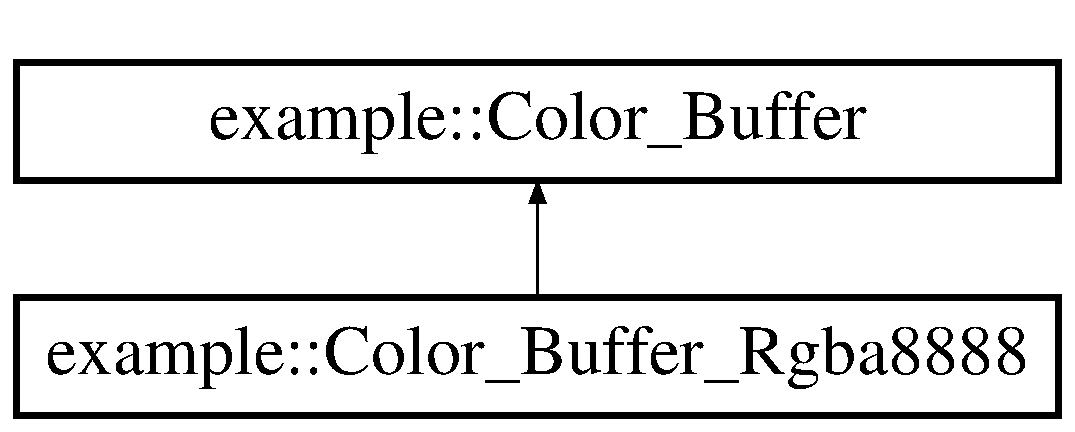
\includegraphics[height=2.000000cm]{classexample_1_1_color___buffer}
\end{center}
\end{figure}
\subsection*{Public Member Functions}
\begin{DoxyCompactItemize}
\item 
\mbox{\hyperlink{classexample_1_1_color___buffer_a44c19770a14b0f8e46e7ceda1df5fc3d}{Color\+\_\+\+Buffer}} (size\+\_\+t \mbox{\hyperlink{classexample_1_1_color___buffer_ab61454d4b35cbba00d2e634d14ed20ac}{width}}, size\+\_\+t \mbox{\hyperlink{classexample_1_1_color___buffer_ae01f4538ee30af1d3072a425c5ad37ac}{height}})
\item 
size\+\_\+t \mbox{\hyperlink{classexample_1_1_color___buffer_a0bbc4a120bc04b512e303baf8330ff82}{get\+\_\+width}} () const
\item 
size\+\_\+t \mbox{\hyperlink{classexample_1_1_color___buffer_a4d1495a260205b83e1bd28dd04c6eda2}{get\+\_\+height}} () const
\item 
int \mbox{\hyperlink{classexample_1_1_color___buffer_ae316a2df43a9ead02cc45170a8d0f7ed}{offset\+\_\+at}} (int x, int y) const
\item 
virtual int \mbox{\hyperlink{classexample_1_1_color___buffer_a76463553dc782f2dc24a61bec708e273}{bits\+\_\+per\+\_\+color}} () const =0
\item 
virtual void \mbox{\hyperlink{classexample_1_1_color___buffer_a3fbfa949ee340ccdb40ad0ce8339b827}{set\+\_\+color}} (int r, int g, int b)=0
\item 
virtual void \mbox{\hyperlink{classexample_1_1_color___buffer_a967ea326ec0889a36db523727a8154b5}{set\+\_\+pixel}} (int x, int y)=0
\item 
virtual void \mbox{\hyperlink{classexample_1_1_color___buffer_a1c919e629ef74e418e1ad416d0a5e85a}{set\+\_\+pixel}} (size\+\_\+t offset)=0
\item 
virtual void \mbox{\hyperlink{classexample_1_1_color___buffer_a793b667028b2eb7efde2cee76066eac7}{gl\+\_\+draw\+\_\+pixels}} (int raster\+\_\+x, int raster\+\_\+y) const =0
\end{DoxyCompactItemize}
\subsection*{Protected Attributes}
\begin{DoxyCompactItemize}
\item 
size\+\_\+t \mbox{\hyperlink{classexample_1_1_color___buffer_ab61454d4b35cbba00d2e634d14ed20ac}{width}}
\item 
size\+\_\+t \mbox{\hyperlink{classexample_1_1_color___buffer_ae01f4538ee30af1d3072a425c5ad37ac}{height}}
\end{DoxyCompactItemize}


\subsection{Constructor \& Destructor Documentation}
\mbox{\Hypertarget{classexample_1_1_color___buffer_a44c19770a14b0f8e46e7ceda1df5fc3d}\label{classexample_1_1_color___buffer_a44c19770a14b0f8e46e7ceda1df5fc3d}} 
\index{example\+::\+Color\+\_\+\+Buffer@{example\+::\+Color\+\_\+\+Buffer}!Color\+\_\+\+Buffer@{Color\+\_\+\+Buffer}}
\index{Color\+\_\+\+Buffer@{Color\+\_\+\+Buffer}!example\+::\+Color\+\_\+\+Buffer@{example\+::\+Color\+\_\+\+Buffer}}
\subsubsection{\texorpdfstring{Color\+\_\+\+Buffer()}{Color\_Buffer()}}
{\footnotesize\ttfamily example\+::\+Color\+\_\+\+Buffer\+::\+Color\+\_\+\+Buffer (\begin{DoxyParamCaption}\item[{size\+\_\+t}]{width,  }\item[{size\+\_\+t}]{height }\end{DoxyParamCaption})\hspace{0.3cm}{\ttfamily [inline]}}



\subsection{Member Function Documentation}
\mbox{\Hypertarget{classexample_1_1_color___buffer_a76463553dc782f2dc24a61bec708e273}\label{classexample_1_1_color___buffer_a76463553dc782f2dc24a61bec708e273}} 
\index{example\+::\+Color\+\_\+\+Buffer@{example\+::\+Color\+\_\+\+Buffer}!bits\+\_\+per\+\_\+color@{bits\+\_\+per\+\_\+color}}
\index{bits\+\_\+per\+\_\+color@{bits\+\_\+per\+\_\+color}!example\+::\+Color\+\_\+\+Buffer@{example\+::\+Color\+\_\+\+Buffer}}
\subsubsection{\texorpdfstring{bits\+\_\+per\+\_\+color()}{bits\_per\_color()}}
{\footnotesize\ttfamily virtual int example\+::\+Color\+\_\+\+Buffer\+::bits\+\_\+per\+\_\+color (\begin{DoxyParamCaption}{ }\end{DoxyParamCaption}) const\hspace{0.3cm}{\ttfamily [pure virtual]}}



Implemented in \mbox{\hyperlink{classexample_1_1_color___buffer___rgba8888_ab2e7a20a9dd24c5dd422d143d9a2d391}{example\+::\+Color\+\_\+\+Buffer\+\_\+\+Rgba8888}}.

\mbox{\Hypertarget{classexample_1_1_color___buffer_a4d1495a260205b83e1bd28dd04c6eda2}\label{classexample_1_1_color___buffer_a4d1495a260205b83e1bd28dd04c6eda2}} 
\index{example\+::\+Color\+\_\+\+Buffer@{example\+::\+Color\+\_\+\+Buffer}!get\+\_\+height@{get\+\_\+height}}
\index{get\+\_\+height@{get\+\_\+height}!example\+::\+Color\+\_\+\+Buffer@{example\+::\+Color\+\_\+\+Buffer}}
\subsubsection{\texorpdfstring{get\+\_\+height()}{get\_height()}}
{\footnotesize\ttfamily size\+\_\+t example\+::\+Color\+\_\+\+Buffer\+::get\+\_\+height (\begin{DoxyParamCaption}{ }\end{DoxyParamCaption}) const\hspace{0.3cm}{\ttfamily [inline]}}

\mbox{\Hypertarget{classexample_1_1_color___buffer_a0bbc4a120bc04b512e303baf8330ff82}\label{classexample_1_1_color___buffer_a0bbc4a120bc04b512e303baf8330ff82}} 
\index{example\+::\+Color\+\_\+\+Buffer@{example\+::\+Color\+\_\+\+Buffer}!get\+\_\+width@{get\+\_\+width}}
\index{get\+\_\+width@{get\+\_\+width}!example\+::\+Color\+\_\+\+Buffer@{example\+::\+Color\+\_\+\+Buffer}}
\subsubsection{\texorpdfstring{get\+\_\+width()}{get\_width()}}
{\footnotesize\ttfamily size\+\_\+t example\+::\+Color\+\_\+\+Buffer\+::get\+\_\+width (\begin{DoxyParamCaption}{ }\end{DoxyParamCaption}) const\hspace{0.3cm}{\ttfamily [inline]}}

\mbox{\Hypertarget{classexample_1_1_color___buffer_a793b667028b2eb7efde2cee76066eac7}\label{classexample_1_1_color___buffer_a793b667028b2eb7efde2cee76066eac7}} 
\index{example\+::\+Color\+\_\+\+Buffer@{example\+::\+Color\+\_\+\+Buffer}!gl\+\_\+draw\+\_\+pixels@{gl\+\_\+draw\+\_\+pixels}}
\index{gl\+\_\+draw\+\_\+pixels@{gl\+\_\+draw\+\_\+pixels}!example\+::\+Color\+\_\+\+Buffer@{example\+::\+Color\+\_\+\+Buffer}}
\subsubsection{\texorpdfstring{gl\+\_\+draw\+\_\+pixels()}{gl\_draw\_pixels()}}
{\footnotesize\ttfamily virtual void example\+::\+Color\+\_\+\+Buffer\+::gl\+\_\+draw\+\_\+pixels (\begin{DoxyParamCaption}\item[{int}]{raster\+\_\+x,  }\item[{int}]{raster\+\_\+y }\end{DoxyParamCaption}) const\hspace{0.3cm}{\ttfamily [pure virtual]}}



Implemented in \mbox{\hyperlink{classexample_1_1_color___buffer___rgba8888_a66e133b6fd196f02a0ba454dd3fc550f}{example\+::\+Color\+\_\+\+Buffer\+\_\+\+Rgba8888}}.

\mbox{\Hypertarget{classexample_1_1_color___buffer_ae316a2df43a9ead02cc45170a8d0f7ed}\label{classexample_1_1_color___buffer_ae316a2df43a9ead02cc45170a8d0f7ed}} 
\index{example\+::\+Color\+\_\+\+Buffer@{example\+::\+Color\+\_\+\+Buffer}!offset\+\_\+at@{offset\+\_\+at}}
\index{offset\+\_\+at@{offset\+\_\+at}!example\+::\+Color\+\_\+\+Buffer@{example\+::\+Color\+\_\+\+Buffer}}
\subsubsection{\texorpdfstring{offset\+\_\+at()}{offset\_at()}}
{\footnotesize\ttfamily int example\+::\+Color\+\_\+\+Buffer\+::offset\+\_\+at (\begin{DoxyParamCaption}\item[{int}]{x,  }\item[{int}]{y }\end{DoxyParamCaption}) const\hspace{0.3cm}{\ttfamily [inline]}}

\mbox{\Hypertarget{classexample_1_1_color___buffer_a3fbfa949ee340ccdb40ad0ce8339b827}\label{classexample_1_1_color___buffer_a3fbfa949ee340ccdb40ad0ce8339b827}} 
\index{example\+::\+Color\+\_\+\+Buffer@{example\+::\+Color\+\_\+\+Buffer}!set\+\_\+color@{set\+\_\+color}}
\index{set\+\_\+color@{set\+\_\+color}!example\+::\+Color\+\_\+\+Buffer@{example\+::\+Color\+\_\+\+Buffer}}
\subsubsection{\texorpdfstring{set\+\_\+color()}{set\_color()}}
{\footnotesize\ttfamily virtual void example\+::\+Color\+\_\+\+Buffer\+::set\+\_\+color (\begin{DoxyParamCaption}\item[{int}]{r,  }\item[{int}]{g,  }\item[{int}]{b }\end{DoxyParamCaption})\hspace{0.3cm}{\ttfamily [pure virtual]}}



Implemented in \mbox{\hyperlink{classexample_1_1_color___buffer___rgba8888_a408bf6adf54fc9958b74d21c8f6da178}{example\+::\+Color\+\_\+\+Buffer\+\_\+\+Rgba8888}}.

\mbox{\Hypertarget{classexample_1_1_color___buffer_a967ea326ec0889a36db523727a8154b5}\label{classexample_1_1_color___buffer_a967ea326ec0889a36db523727a8154b5}} 
\index{example\+::\+Color\+\_\+\+Buffer@{example\+::\+Color\+\_\+\+Buffer}!set\+\_\+pixel@{set\+\_\+pixel}}
\index{set\+\_\+pixel@{set\+\_\+pixel}!example\+::\+Color\+\_\+\+Buffer@{example\+::\+Color\+\_\+\+Buffer}}
\subsubsection{\texorpdfstring{set\+\_\+pixel()}{set\_pixel()}\hspace{0.1cm}{\footnotesize\ttfamily [1/2]}}
{\footnotesize\ttfamily virtual void example\+::\+Color\+\_\+\+Buffer\+::set\+\_\+pixel (\begin{DoxyParamCaption}\item[{int}]{x,  }\item[{int}]{y }\end{DoxyParamCaption})\hspace{0.3cm}{\ttfamily [pure virtual]}}



Implemented in \mbox{\hyperlink{classexample_1_1_color___buffer___rgba8888_aceb94fbc6797177c5a401f4d10d56766}{example\+::\+Color\+\_\+\+Buffer\+\_\+\+Rgba8888}}.

\mbox{\Hypertarget{classexample_1_1_color___buffer_a1c919e629ef74e418e1ad416d0a5e85a}\label{classexample_1_1_color___buffer_a1c919e629ef74e418e1ad416d0a5e85a}} 
\index{example\+::\+Color\+\_\+\+Buffer@{example\+::\+Color\+\_\+\+Buffer}!set\+\_\+pixel@{set\+\_\+pixel}}
\index{set\+\_\+pixel@{set\+\_\+pixel}!example\+::\+Color\+\_\+\+Buffer@{example\+::\+Color\+\_\+\+Buffer}}
\subsubsection{\texorpdfstring{set\+\_\+pixel()}{set\_pixel()}\hspace{0.1cm}{\footnotesize\ttfamily [2/2]}}
{\footnotesize\ttfamily virtual void example\+::\+Color\+\_\+\+Buffer\+::set\+\_\+pixel (\begin{DoxyParamCaption}\item[{size\+\_\+t}]{offset }\end{DoxyParamCaption})\hspace{0.3cm}{\ttfamily [pure virtual]}}



Implemented in \mbox{\hyperlink{classexample_1_1_color___buffer___rgba8888_ac741fa7bca9b980a475e6f7033b64347}{example\+::\+Color\+\_\+\+Buffer\+\_\+\+Rgba8888}}.



\subsection{Member Data Documentation}
\mbox{\Hypertarget{classexample_1_1_color___buffer_ae01f4538ee30af1d3072a425c5ad37ac}\label{classexample_1_1_color___buffer_ae01f4538ee30af1d3072a425c5ad37ac}} 
\index{example\+::\+Color\+\_\+\+Buffer@{example\+::\+Color\+\_\+\+Buffer}!height@{height}}
\index{height@{height}!example\+::\+Color\+\_\+\+Buffer@{example\+::\+Color\+\_\+\+Buffer}}
\subsubsection{\texorpdfstring{height}{height}}
{\footnotesize\ttfamily size\+\_\+t example\+::\+Color\+\_\+\+Buffer\+::height\hspace{0.3cm}{\ttfamily [protected]}}

\mbox{\Hypertarget{classexample_1_1_color___buffer_ab61454d4b35cbba00d2e634d14ed20ac}\label{classexample_1_1_color___buffer_ab61454d4b35cbba00d2e634d14ed20ac}} 
\index{example\+::\+Color\+\_\+\+Buffer@{example\+::\+Color\+\_\+\+Buffer}!width@{width}}
\index{width@{width}!example\+::\+Color\+\_\+\+Buffer@{example\+::\+Color\+\_\+\+Buffer}}
\subsubsection{\texorpdfstring{width}{width}}
{\footnotesize\ttfamily size\+\_\+t example\+::\+Color\+\_\+\+Buffer\+::width\hspace{0.3cm}{\ttfamily [protected]}}



The documentation for this class was generated from the following file\+:\begin{DoxyCompactItemize}
\item 
D\+:/\+Git\+Kraken/3\+D\+Av\+\_\+2/src/\mbox{\hyperlink{_color___buffer_8hpp}{Color\+\_\+\+Buffer.\+hpp}}\end{DoxyCompactItemize}

\hypertarget{classexample_1_1_color___buffer___rgba8888}{}\section{example\+:\+:Color\+\_\+\+Buffer\+\_\+\+Rgba8888 Class Reference}
\label{classexample_1_1_color___buffer___rgba8888}\index{example\+::\+Color\+\_\+\+Buffer\+\_\+\+Rgba8888@{example\+::\+Color\+\_\+\+Buffer\+\_\+\+Rgba8888}}


{\ttfamily \#include $<$Color\+\_\+\+Buffer\+\_\+\+Rgba8888.\+hpp$>$}

Inheritance diagram for example\+:\+:Color\+\_\+\+Buffer\+\_\+\+Rgba8888\+:\begin{figure}[H]
\begin{center}
\leavevmode
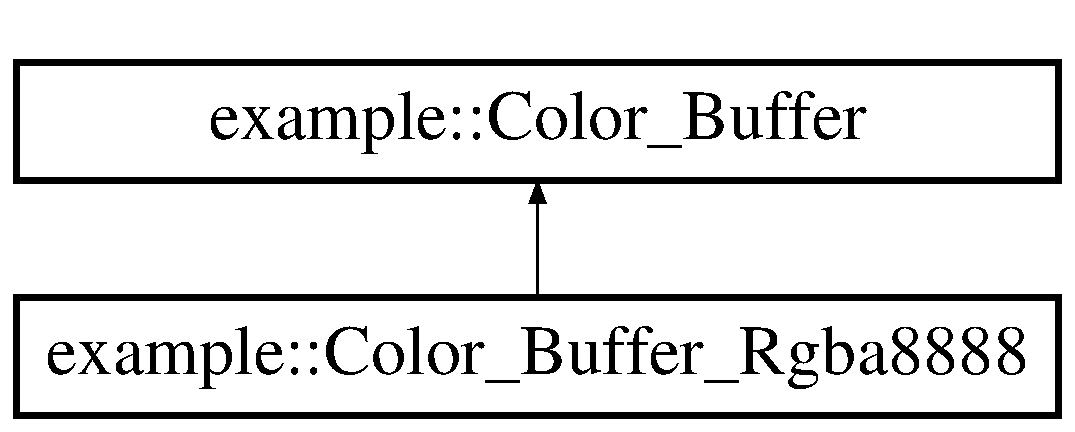
\includegraphics[height=2.000000cm]{classexample_1_1_color___buffer___rgba8888}
\end{center}
\end{figure}
\subsection*{Classes}
\begin{DoxyCompactItemize}
\item 
struct \mbox{\hyperlink{structexample_1_1_color___buffer___rgba8888_1_1_color}{Color}}
\end{DoxyCompactItemize}
\subsection*{Public Types}
\begin{DoxyCompactItemize}
\item 
typedef std\+::vector$<$ \mbox{\hyperlink{structexample_1_1_color___buffer___rgba8888_1_1_color}{Color}} $>$ \mbox{\hyperlink{classexample_1_1_color___buffer___rgba8888_ac6bfcddbbeeb02961b8724d9f5e10033}{Buffer}}
\end{DoxyCompactItemize}
\subsection*{Public Member Functions}
\begin{DoxyCompactItemize}
\item 
\mbox{\hyperlink{classexample_1_1_color___buffer___rgba8888_aa5397ac3ceb62d95d0f4773205d98177}{Color\+\_\+\+Buffer\+\_\+\+Rgba8888}} (size\+\_\+t \mbox{\hyperlink{classexample_1_1_color___buffer_ab61454d4b35cbba00d2e634d14ed20ac}{width}}, size\+\_\+t \mbox{\hyperlink{classexample_1_1_color___buffer_ae01f4538ee30af1d3072a425c5ad37ac}{height}})
\item 
\mbox{\hyperlink{structexample_1_1_color___buffer___rgba8888_1_1_color}{Color}} $\ast$ \mbox{\hyperlink{classexample_1_1_color___buffer___rgba8888_aec3a6be699750106d4a9ccd5f7f75f74}{colors}} ()
\item 
const \mbox{\hyperlink{structexample_1_1_color___buffer___rgba8888_1_1_color}{Color}} $\ast$ \mbox{\hyperlink{classexample_1_1_color___buffer___rgba8888_aea57e24bede44fa736473824e8f14a1f}{colors}} () const
\item 
int \mbox{\hyperlink{classexample_1_1_color___buffer___rgba8888_ab2e7a20a9dd24c5dd422d143d9a2d391}{bits\+\_\+per\+\_\+color}} () const
\item 
size\+\_\+t \mbox{\hyperlink{classexample_1_1_color___buffer___rgba8888_a635f30dda6b8e1851b444ff6e0d2a092}{size}} () const
\item 
void \mbox{\hyperlink{classexample_1_1_color___buffer___rgba8888_a408bf6adf54fc9958b74d21c8f6da178}{set\+\_\+color}} (int r, int g, int b)
\item 
void \mbox{\hyperlink{classexample_1_1_color___buffer___rgba8888_a5033d0d18293c92936fd2ff5318e3f0f}{set\+\_\+color}} (const \mbox{\hyperlink{structexample_1_1_color___buffer___rgba8888_1_1_color}{Color}} \&new\+\_\+color)
\item 
void \mbox{\hyperlink{classexample_1_1_color___buffer___rgba8888_ac741fa7bca9b980a475e6f7033b64347}{set\+\_\+pixel}} (size\+\_\+t offset)
\item 
void \mbox{\hyperlink{classexample_1_1_color___buffer___rgba8888_aceb94fbc6797177c5a401f4d10d56766}{set\+\_\+pixel}} (int x, int y)
\item 
uint8\+\_\+t \mbox{\hyperlink{classexample_1_1_color___buffer___rgba8888_afd80c65a9ba578b74f044ae8927e5a97}{get\+\_\+pixel}} (int x, int y)
\begin{DoxyCompactList}\small\item\em No terminado. \end{DoxyCompactList}\item 
void \mbox{\hyperlink{classexample_1_1_color___buffer___rgba8888_a66e133b6fd196f02a0ba454dd3fc550f}{gl\+\_\+draw\+\_\+pixels}} (int raster\+\_\+x, int raster\+\_\+y) const
\end{DoxyCompactItemize}
\subsection*{Additional Inherited Members}


\subsection{Member Typedef Documentation}
\mbox{\Hypertarget{classexample_1_1_color___buffer___rgba8888_ac6bfcddbbeeb02961b8724d9f5e10033}\label{classexample_1_1_color___buffer___rgba8888_ac6bfcddbbeeb02961b8724d9f5e10033}} 
\index{example\+::\+Color\+\_\+\+Buffer\+\_\+\+Rgba8888@{example\+::\+Color\+\_\+\+Buffer\+\_\+\+Rgba8888}!Buffer@{Buffer}}
\index{Buffer@{Buffer}!example\+::\+Color\+\_\+\+Buffer\+\_\+\+Rgba8888@{example\+::\+Color\+\_\+\+Buffer\+\_\+\+Rgba8888}}
\subsubsection{\texorpdfstring{Buffer}{Buffer}}
{\footnotesize\ttfamily typedef std\+::vector$<$ \mbox{\hyperlink{structexample_1_1_color___buffer___rgba8888_1_1_color}{Color}} $>$ \mbox{\hyperlink{classexample_1_1_color___buffer___rgba8888_ac6bfcddbbeeb02961b8724d9f5e10033}{example\+::\+Color\+\_\+\+Buffer\+\_\+\+Rgba8888\+::\+Buffer}}}



\subsection{Constructor \& Destructor Documentation}
\mbox{\Hypertarget{classexample_1_1_color___buffer___rgba8888_aa5397ac3ceb62d95d0f4773205d98177}\label{classexample_1_1_color___buffer___rgba8888_aa5397ac3ceb62d95d0f4773205d98177}} 
\index{example\+::\+Color\+\_\+\+Buffer\+\_\+\+Rgba8888@{example\+::\+Color\+\_\+\+Buffer\+\_\+\+Rgba8888}!Color\+\_\+\+Buffer\+\_\+\+Rgba8888@{Color\+\_\+\+Buffer\+\_\+\+Rgba8888}}
\index{Color\+\_\+\+Buffer\+\_\+\+Rgba8888@{Color\+\_\+\+Buffer\+\_\+\+Rgba8888}!example\+::\+Color\+\_\+\+Buffer\+\_\+\+Rgba8888@{example\+::\+Color\+\_\+\+Buffer\+\_\+\+Rgba8888}}
\subsubsection{\texorpdfstring{Color\+\_\+\+Buffer\+\_\+\+Rgba8888()}{Color\_Buffer\_Rgba8888()}}
{\footnotesize\ttfamily example\+::\+Color\+\_\+\+Buffer\+\_\+\+Rgba8888\+::\+Color\+\_\+\+Buffer\+\_\+\+Rgba8888 (\begin{DoxyParamCaption}\item[{size\+\_\+t}]{width,  }\item[{size\+\_\+t}]{height }\end{DoxyParamCaption})\hspace{0.3cm}{\ttfamily [inline]}}



\subsection{Member Function Documentation}
\mbox{\Hypertarget{classexample_1_1_color___buffer___rgba8888_ab2e7a20a9dd24c5dd422d143d9a2d391}\label{classexample_1_1_color___buffer___rgba8888_ab2e7a20a9dd24c5dd422d143d9a2d391}} 
\index{example\+::\+Color\+\_\+\+Buffer\+\_\+\+Rgba8888@{example\+::\+Color\+\_\+\+Buffer\+\_\+\+Rgba8888}!bits\+\_\+per\+\_\+color@{bits\+\_\+per\+\_\+color}}
\index{bits\+\_\+per\+\_\+color@{bits\+\_\+per\+\_\+color}!example\+::\+Color\+\_\+\+Buffer\+\_\+\+Rgba8888@{example\+::\+Color\+\_\+\+Buffer\+\_\+\+Rgba8888}}
\subsubsection{\texorpdfstring{bits\+\_\+per\+\_\+color()}{bits\_per\_color()}}
{\footnotesize\ttfamily int example\+::\+Color\+\_\+\+Buffer\+\_\+\+Rgba8888\+::bits\+\_\+per\+\_\+color (\begin{DoxyParamCaption}{ }\end{DoxyParamCaption}) const\hspace{0.3cm}{\ttfamily [inline]}, {\ttfamily [virtual]}}



Implements \mbox{\hyperlink{classexample_1_1_color___buffer_a76463553dc782f2dc24a61bec708e273}{example\+::\+Color\+\_\+\+Buffer}}.

\mbox{\Hypertarget{classexample_1_1_color___buffer___rgba8888_aec3a6be699750106d4a9ccd5f7f75f74}\label{classexample_1_1_color___buffer___rgba8888_aec3a6be699750106d4a9ccd5f7f75f74}} 
\index{example\+::\+Color\+\_\+\+Buffer\+\_\+\+Rgba8888@{example\+::\+Color\+\_\+\+Buffer\+\_\+\+Rgba8888}!colors@{colors}}
\index{colors@{colors}!example\+::\+Color\+\_\+\+Buffer\+\_\+\+Rgba8888@{example\+::\+Color\+\_\+\+Buffer\+\_\+\+Rgba8888}}
\subsubsection{\texorpdfstring{colors()}{colors()}\hspace{0.1cm}{\footnotesize\ttfamily [1/2]}}
{\footnotesize\ttfamily \mbox{\hyperlink{structexample_1_1_color___buffer___rgba8888_1_1_color}{Color}}$\ast$ example\+::\+Color\+\_\+\+Buffer\+\_\+\+Rgba8888\+::colors (\begin{DoxyParamCaption}{ }\end{DoxyParamCaption})\hspace{0.3cm}{\ttfamily [inline]}}

\mbox{\Hypertarget{classexample_1_1_color___buffer___rgba8888_aea57e24bede44fa736473824e8f14a1f}\label{classexample_1_1_color___buffer___rgba8888_aea57e24bede44fa736473824e8f14a1f}} 
\index{example\+::\+Color\+\_\+\+Buffer\+\_\+\+Rgba8888@{example\+::\+Color\+\_\+\+Buffer\+\_\+\+Rgba8888}!colors@{colors}}
\index{colors@{colors}!example\+::\+Color\+\_\+\+Buffer\+\_\+\+Rgba8888@{example\+::\+Color\+\_\+\+Buffer\+\_\+\+Rgba8888}}
\subsubsection{\texorpdfstring{colors()}{colors()}\hspace{0.1cm}{\footnotesize\ttfamily [2/2]}}
{\footnotesize\ttfamily const \mbox{\hyperlink{structexample_1_1_color___buffer___rgba8888_1_1_color}{Color}}$\ast$ example\+::\+Color\+\_\+\+Buffer\+\_\+\+Rgba8888\+::colors (\begin{DoxyParamCaption}{ }\end{DoxyParamCaption}) const\hspace{0.3cm}{\ttfamily [inline]}}

\mbox{\Hypertarget{classexample_1_1_color___buffer___rgba8888_afd80c65a9ba578b74f044ae8927e5a97}\label{classexample_1_1_color___buffer___rgba8888_afd80c65a9ba578b74f044ae8927e5a97}} 
\index{example\+::\+Color\+\_\+\+Buffer\+\_\+\+Rgba8888@{example\+::\+Color\+\_\+\+Buffer\+\_\+\+Rgba8888}!get\+\_\+pixel@{get\+\_\+pixel}}
\index{get\+\_\+pixel@{get\+\_\+pixel}!example\+::\+Color\+\_\+\+Buffer\+\_\+\+Rgba8888@{example\+::\+Color\+\_\+\+Buffer\+\_\+\+Rgba8888}}
\subsubsection{\texorpdfstring{get\+\_\+pixel()}{get\_pixel()}}
{\footnotesize\ttfamily uint8\+\_\+t example\+::\+Color\+\_\+\+Buffer\+\_\+\+Rgba8888\+::get\+\_\+pixel (\begin{DoxyParamCaption}\item[{int}]{x,  }\item[{int}]{y }\end{DoxyParamCaption})\hspace{0.3cm}{\ttfamily [inline]}}



No terminado. 

\mbox{\Hypertarget{classexample_1_1_color___buffer___rgba8888_a66e133b6fd196f02a0ba454dd3fc550f}\label{classexample_1_1_color___buffer___rgba8888_a66e133b6fd196f02a0ba454dd3fc550f}} 
\index{example\+::\+Color\+\_\+\+Buffer\+\_\+\+Rgba8888@{example\+::\+Color\+\_\+\+Buffer\+\_\+\+Rgba8888}!gl\+\_\+draw\+\_\+pixels@{gl\+\_\+draw\+\_\+pixels}}
\index{gl\+\_\+draw\+\_\+pixels@{gl\+\_\+draw\+\_\+pixels}!example\+::\+Color\+\_\+\+Buffer\+\_\+\+Rgba8888@{example\+::\+Color\+\_\+\+Buffer\+\_\+\+Rgba8888}}
\subsubsection{\texorpdfstring{gl\+\_\+draw\+\_\+pixels()}{gl\_draw\_pixels()}}
{\footnotesize\ttfamily void example\+::\+Color\+\_\+\+Buffer\+\_\+\+Rgba8888\+::gl\+\_\+draw\+\_\+pixels (\begin{DoxyParamCaption}\item[{int}]{raster\+\_\+x,  }\item[{int}]{raster\+\_\+y }\end{DoxyParamCaption}) const\hspace{0.3cm}{\ttfamily [inline]}, {\ttfamily [virtual]}}



Implements \mbox{\hyperlink{classexample_1_1_color___buffer_a793b667028b2eb7efde2cee76066eac7}{example\+::\+Color\+\_\+\+Buffer}}.

\mbox{\Hypertarget{classexample_1_1_color___buffer___rgba8888_a408bf6adf54fc9958b74d21c8f6da178}\label{classexample_1_1_color___buffer___rgba8888_a408bf6adf54fc9958b74d21c8f6da178}} 
\index{example\+::\+Color\+\_\+\+Buffer\+\_\+\+Rgba8888@{example\+::\+Color\+\_\+\+Buffer\+\_\+\+Rgba8888}!set\+\_\+color@{set\+\_\+color}}
\index{set\+\_\+color@{set\+\_\+color}!example\+::\+Color\+\_\+\+Buffer\+\_\+\+Rgba8888@{example\+::\+Color\+\_\+\+Buffer\+\_\+\+Rgba8888}}
\subsubsection{\texorpdfstring{set\+\_\+color()}{set\_color()}\hspace{0.1cm}{\footnotesize\ttfamily [1/2]}}
{\footnotesize\ttfamily void example\+::\+Color\+\_\+\+Buffer\+\_\+\+Rgba8888\+::set\+\_\+color (\begin{DoxyParamCaption}\item[{int}]{r,  }\item[{int}]{g,  }\item[{int}]{b }\end{DoxyParamCaption})\hspace{0.3cm}{\ttfamily [inline]}, {\ttfamily [virtual]}}



Implements \mbox{\hyperlink{classexample_1_1_color___buffer_a3fbfa949ee340ccdb40ad0ce8339b827}{example\+::\+Color\+\_\+\+Buffer}}.

\mbox{\Hypertarget{classexample_1_1_color___buffer___rgba8888_a5033d0d18293c92936fd2ff5318e3f0f}\label{classexample_1_1_color___buffer___rgba8888_a5033d0d18293c92936fd2ff5318e3f0f}} 
\index{example\+::\+Color\+\_\+\+Buffer\+\_\+\+Rgba8888@{example\+::\+Color\+\_\+\+Buffer\+\_\+\+Rgba8888}!set\+\_\+color@{set\+\_\+color}}
\index{set\+\_\+color@{set\+\_\+color}!example\+::\+Color\+\_\+\+Buffer\+\_\+\+Rgba8888@{example\+::\+Color\+\_\+\+Buffer\+\_\+\+Rgba8888}}
\subsubsection{\texorpdfstring{set\+\_\+color()}{set\_color()}\hspace{0.1cm}{\footnotesize\ttfamily [2/2]}}
{\footnotesize\ttfamily void example\+::\+Color\+\_\+\+Buffer\+\_\+\+Rgba8888\+::set\+\_\+color (\begin{DoxyParamCaption}\item[{const \mbox{\hyperlink{structexample_1_1_color___buffer___rgba8888_1_1_color}{Color}} \&}]{new\+\_\+color }\end{DoxyParamCaption})\hspace{0.3cm}{\ttfamily [inline]}}

\mbox{\Hypertarget{classexample_1_1_color___buffer___rgba8888_ac741fa7bca9b980a475e6f7033b64347}\label{classexample_1_1_color___buffer___rgba8888_ac741fa7bca9b980a475e6f7033b64347}} 
\index{example\+::\+Color\+\_\+\+Buffer\+\_\+\+Rgba8888@{example\+::\+Color\+\_\+\+Buffer\+\_\+\+Rgba8888}!set\+\_\+pixel@{set\+\_\+pixel}}
\index{set\+\_\+pixel@{set\+\_\+pixel}!example\+::\+Color\+\_\+\+Buffer\+\_\+\+Rgba8888@{example\+::\+Color\+\_\+\+Buffer\+\_\+\+Rgba8888}}
\subsubsection{\texorpdfstring{set\+\_\+pixel()}{set\_pixel()}\hspace{0.1cm}{\footnotesize\ttfamily [1/2]}}
{\footnotesize\ttfamily void example\+::\+Color\+\_\+\+Buffer\+\_\+\+Rgba8888\+::set\+\_\+pixel (\begin{DoxyParamCaption}\item[{size\+\_\+t}]{offset }\end{DoxyParamCaption})\hspace{0.3cm}{\ttfamily [inline]}, {\ttfamily [virtual]}}



Implements \mbox{\hyperlink{classexample_1_1_color___buffer_a1c919e629ef74e418e1ad416d0a5e85a}{example\+::\+Color\+\_\+\+Buffer}}.

\mbox{\Hypertarget{classexample_1_1_color___buffer___rgba8888_aceb94fbc6797177c5a401f4d10d56766}\label{classexample_1_1_color___buffer___rgba8888_aceb94fbc6797177c5a401f4d10d56766}} 
\index{example\+::\+Color\+\_\+\+Buffer\+\_\+\+Rgba8888@{example\+::\+Color\+\_\+\+Buffer\+\_\+\+Rgba8888}!set\+\_\+pixel@{set\+\_\+pixel}}
\index{set\+\_\+pixel@{set\+\_\+pixel}!example\+::\+Color\+\_\+\+Buffer\+\_\+\+Rgba8888@{example\+::\+Color\+\_\+\+Buffer\+\_\+\+Rgba8888}}
\subsubsection{\texorpdfstring{set\+\_\+pixel()}{set\_pixel()}\hspace{0.1cm}{\footnotesize\ttfamily [2/2]}}
{\footnotesize\ttfamily void example\+::\+Color\+\_\+\+Buffer\+\_\+\+Rgba8888\+::set\+\_\+pixel (\begin{DoxyParamCaption}\item[{int}]{x,  }\item[{int}]{y }\end{DoxyParamCaption})\hspace{0.3cm}{\ttfamily [inline]}, {\ttfamily [virtual]}}



Implements \mbox{\hyperlink{classexample_1_1_color___buffer_a967ea326ec0889a36db523727a8154b5}{example\+::\+Color\+\_\+\+Buffer}}.

\mbox{\Hypertarget{classexample_1_1_color___buffer___rgba8888_a635f30dda6b8e1851b444ff6e0d2a092}\label{classexample_1_1_color___buffer___rgba8888_a635f30dda6b8e1851b444ff6e0d2a092}} 
\index{example\+::\+Color\+\_\+\+Buffer\+\_\+\+Rgba8888@{example\+::\+Color\+\_\+\+Buffer\+\_\+\+Rgba8888}!size@{size}}
\index{size@{size}!example\+::\+Color\+\_\+\+Buffer\+\_\+\+Rgba8888@{example\+::\+Color\+\_\+\+Buffer\+\_\+\+Rgba8888}}
\subsubsection{\texorpdfstring{size()}{size()}}
{\footnotesize\ttfamily size\+\_\+t example\+::\+Color\+\_\+\+Buffer\+\_\+\+Rgba8888\+::size (\begin{DoxyParamCaption}{ }\end{DoxyParamCaption}) const\hspace{0.3cm}{\ttfamily [inline]}}



The documentation for this class was generated from the following file\+:\begin{DoxyCompactItemize}
\item 
D\+:/\+Git\+Kraken/3\+D\+Av\+\_\+2/src/\mbox{\hyperlink{_color___buffer___rgba8888_8hpp}{Color\+\_\+\+Buffer\+\_\+\+Rgba8888.\+hpp}}\end{DoxyCompactItemize}

\hypertarget{classexample_1_1_cube}{}\section{example\+:\+:Cube Class Reference}
\label{classexample_1_1_cube}\index{example\+::\+Cube@{example\+::\+Cube}}


{\ttfamily \#include $<$Cube.\+hpp$>$}

\subsection*{Public Member Functions}
\begin{DoxyCompactItemize}
\item 
\mbox{\hyperlink{classexample_1_1_cube_a3be7fbbad6d33b8ca68487fea7e20bdf}{Cube}} ()
\item 
\mbox{\hyperlink{classexample_1_1_cube_ab82f621c8aeb1ce7ccd72afd605d6b7a}{$\sim$\+Cube}} ()
\item 
void \mbox{\hyperlink{classexample_1_1_cube_a9f968872ab6a7ee0362e49a0c5f4e8b6}{render}} ()
\end{DoxyCompactItemize}


\subsection{Constructor \& Destructor Documentation}
\mbox{\Hypertarget{classexample_1_1_cube_a3be7fbbad6d33b8ca68487fea7e20bdf}\label{classexample_1_1_cube_a3be7fbbad6d33b8ca68487fea7e20bdf}} 
\index{example\+::\+Cube@{example\+::\+Cube}!Cube@{Cube}}
\index{Cube@{Cube}!example\+::\+Cube@{example\+::\+Cube}}
\subsubsection{\texorpdfstring{Cube()}{Cube()}}
{\footnotesize\ttfamily example\+::\+Cube\+::\+Cube (\begin{DoxyParamCaption}{ }\end{DoxyParamCaption})}

\mbox{\Hypertarget{classexample_1_1_cube_ab82f621c8aeb1ce7ccd72afd605d6b7a}\label{classexample_1_1_cube_ab82f621c8aeb1ce7ccd72afd605d6b7a}} 
\index{example\+::\+Cube@{example\+::\+Cube}!````~Cube@{$\sim$\+Cube}}
\index{````~Cube@{$\sim$\+Cube}!example\+::\+Cube@{example\+::\+Cube}}
\subsubsection{\texorpdfstring{$\sim$\+Cube()}{~Cube()}}
{\footnotesize\ttfamily example\+::\+Cube\+::$\sim$\+Cube (\begin{DoxyParamCaption}{ }\end{DoxyParamCaption})}



\subsection{Member Function Documentation}
\mbox{\Hypertarget{classexample_1_1_cube_a9f968872ab6a7ee0362e49a0c5f4e8b6}\label{classexample_1_1_cube_a9f968872ab6a7ee0362e49a0c5f4e8b6}} 
\index{example\+::\+Cube@{example\+::\+Cube}!render@{render}}
\index{render@{render}!example\+::\+Cube@{example\+::\+Cube}}
\subsubsection{\texorpdfstring{render()}{render()}}
{\footnotesize\ttfamily void example\+::\+Cube\+::render (\begin{DoxyParamCaption}{ }\end{DoxyParamCaption})}



The documentation for this class was generated from the following files\+:\begin{DoxyCompactItemize}
\item 
D\+:/\+Git\+Kraken/3\+D\+Av\+\_\+2/src/\mbox{\hyperlink{_cube_8hpp}{Cube.\+hpp}}\item 
D\+:/\+Git\+Kraken/3\+D\+Av\+\_\+2/src/\mbox{\hyperlink{_cube_8cpp}{Cube.\+cpp}}\end{DoxyCompactItemize}

\hypertarget{classexample_1_1_elevation___mesh}{}\section{example\+:\+:Elevation\+\_\+\+Mesh Class Reference}
\label{classexample_1_1_elevation___mesh}\index{example\+::\+Elevation\+\_\+\+Mesh@{example\+::\+Elevation\+\_\+\+Mesh}}


{\ttfamily \#include $<$Elevation\+\_\+\+Mesh.\+hpp$>$}

Inheritance diagram for example\+:\+:Elevation\+\_\+\+Mesh\+:\begin{figure}[H]
\begin{center}
\leavevmode
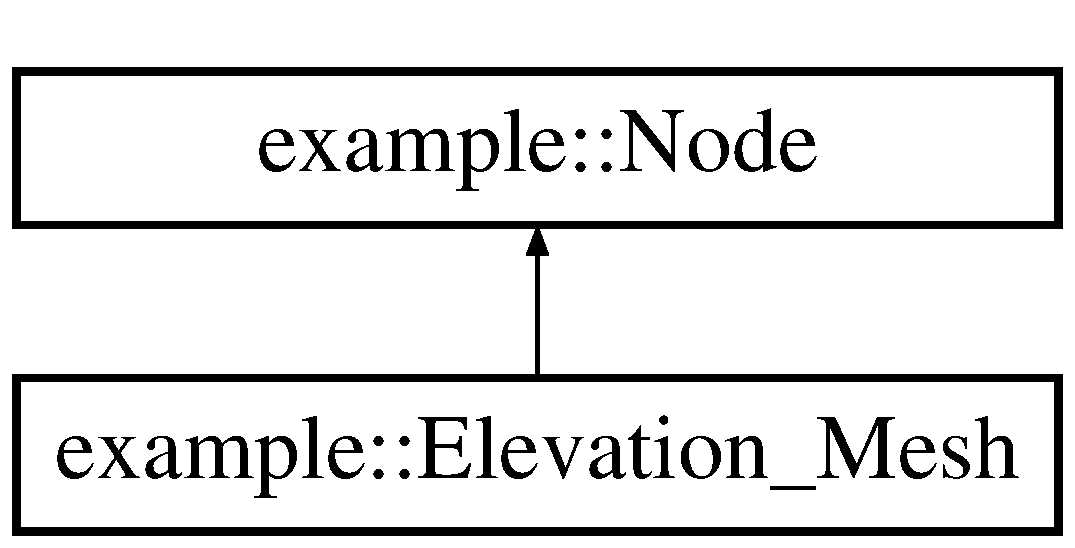
\includegraphics[height=2.000000cm]{classexample_1_1_elevation___mesh}
\end{center}
\end{figure}
\subsection*{Public Member Functions}
\begin{DoxyCompactItemize}
\item 
\mbox{\hyperlink{classexample_1_1_elevation___mesh_a631c220a9e5c04f1c84b5301329c3791}{Elevation\+\_\+\+Mesh}} (int cols, int rows, float width, float depth, float elevation, shared\+\_\+ptr$<$ \mbox{\hyperlink{classexample_1_1_shader___program}{Shader\+\_\+\+Program}} $>$ shader)
\item 
\mbox{\hyperlink{classexample_1_1_elevation___mesh_a64aaa59bc4b872cf5180e444d3cb1073}{$\sim$\+Elevation\+\_\+\+Mesh}} ()
\item 
glm\+::vec3 \mbox{\hyperlink{classexample_1_1_elevation___mesh_a3a4637a65ae4c1a7d0f051d26b1f78d8}{calculate\+\_\+normal}} (const Point3f \&p0, const Point3f \&p1, const Point3f \&p2)
\item 
glm\+::vec3 \mbox{\hyperlink{classexample_1_1_elevation___mesh_aee6583fd55f431f0a6b8dc8e99b6db94}{calculate\+\_\+normal}} (const Point3f \&p0, const Point3f \&p1, const Point3f \&p2, const Point3f \&p3, const Point3f \&p4, const Point3f \&p5, const Point3f \&p6, const Point3f \&p7, const Point3f \&p8)
\item 
void \mbox{\hyperlink{classexample_1_1_elevation___mesh_a6af1c74193b5e68d638382caa08f1d1a}{render}} (const glm\+::mat4 \&parent\+\_\+model\+\_\+view) override
\end{DoxyCompactItemize}
\subsection*{Additional Inherited Members}


\subsection{Constructor \& Destructor Documentation}
\mbox{\Hypertarget{classexample_1_1_elevation___mesh_a631c220a9e5c04f1c84b5301329c3791}\label{classexample_1_1_elevation___mesh_a631c220a9e5c04f1c84b5301329c3791}} 
\index{example\+::\+Elevation\+\_\+\+Mesh@{example\+::\+Elevation\+\_\+\+Mesh}!Elevation\+\_\+\+Mesh@{Elevation\+\_\+\+Mesh}}
\index{Elevation\+\_\+\+Mesh@{Elevation\+\_\+\+Mesh}!example\+::\+Elevation\+\_\+\+Mesh@{example\+::\+Elevation\+\_\+\+Mesh}}
\subsubsection{\texorpdfstring{Elevation\+\_\+\+Mesh()}{Elevation\_Mesh()}}
{\footnotesize\ttfamily example\+::\+Elevation\+\_\+\+Mesh\+::\+Elevation\+\_\+\+Mesh (\begin{DoxyParamCaption}\item[{int}]{cols,  }\item[{int}]{rows,  }\item[{float}]{width,  }\item[{float}]{depth,  }\item[{float}]{elevation,  }\item[{shared\+\_\+ptr$<$ \mbox{\hyperlink{classexample_1_1_shader___program}{Shader\+\_\+\+Program}} $>$}]{shader }\end{DoxyParamCaption})}

\mbox{\Hypertarget{classexample_1_1_elevation___mesh_a64aaa59bc4b872cf5180e444d3cb1073}\label{classexample_1_1_elevation___mesh_a64aaa59bc4b872cf5180e444d3cb1073}} 
\index{example\+::\+Elevation\+\_\+\+Mesh@{example\+::\+Elevation\+\_\+\+Mesh}!````~Elevation\+\_\+\+Mesh@{$\sim$\+Elevation\+\_\+\+Mesh}}
\index{````~Elevation\+\_\+\+Mesh@{$\sim$\+Elevation\+\_\+\+Mesh}!example\+::\+Elevation\+\_\+\+Mesh@{example\+::\+Elevation\+\_\+\+Mesh}}
\subsubsection{\texorpdfstring{$\sim$\+Elevation\+\_\+\+Mesh()}{~Elevation\_Mesh()}}
{\footnotesize\ttfamily example\+::\+Elevation\+\_\+\+Mesh\+::$\sim$\+Elevation\+\_\+\+Mesh (\begin{DoxyParamCaption}{ }\end{DoxyParamCaption})}



\subsection{Member Function Documentation}
\mbox{\Hypertarget{classexample_1_1_elevation___mesh_a3a4637a65ae4c1a7d0f051d26b1f78d8}\label{classexample_1_1_elevation___mesh_a3a4637a65ae4c1a7d0f051d26b1f78d8}} 
\index{example\+::\+Elevation\+\_\+\+Mesh@{example\+::\+Elevation\+\_\+\+Mesh}!calculate\+\_\+normal@{calculate\+\_\+normal}}
\index{calculate\+\_\+normal@{calculate\+\_\+normal}!example\+::\+Elevation\+\_\+\+Mesh@{example\+::\+Elevation\+\_\+\+Mesh}}
\subsubsection{\texorpdfstring{calculate\+\_\+normal()}{calculate\_normal()}\hspace{0.1cm}{\footnotesize\ttfamily [1/2]}}
{\footnotesize\ttfamily glm\+::vec3 example\+::\+Elevation\+\_\+\+Mesh\+::calculate\+\_\+normal (\begin{DoxyParamCaption}\item[{const Point3f \&}]{p0,  }\item[{const Point3f \&}]{p1,  }\item[{const Point3f \&}]{p2 }\end{DoxyParamCaption})}

\mbox{\Hypertarget{classexample_1_1_elevation___mesh_aee6583fd55f431f0a6b8dc8e99b6db94}\label{classexample_1_1_elevation___mesh_aee6583fd55f431f0a6b8dc8e99b6db94}} 
\index{example\+::\+Elevation\+\_\+\+Mesh@{example\+::\+Elevation\+\_\+\+Mesh}!calculate\+\_\+normal@{calculate\+\_\+normal}}
\index{calculate\+\_\+normal@{calculate\+\_\+normal}!example\+::\+Elevation\+\_\+\+Mesh@{example\+::\+Elevation\+\_\+\+Mesh}}
\subsubsection{\texorpdfstring{calculate\+\_\+normal()}{calculate\_normal()}\hspace{0.1cm}{\footnotesize\ttfamily [2/2]}}
{\footnotesize\ttfamily glm\+::vec3 example\+::\+Elevation\+\_\+\+Mesh\+::calculate\+\_\+normal (\begin{DoxyParamCaption}\item[{const Point3f \&}]{p0,  }\item[{const Point3f \&}]{p1,  }\item[{const Point3f \&}]{p2,  }\item[{const Point3f \&}]{p3,  }\item[{const Point3f \&}]{p4,  }\item[{const Point3f \&}]{p5,  }\item[{const Point3f \&}]{p6,  }\item[{const Point3f \&}]{p7,  }\item[{const Point3f \&}]{p8 }\end{DoxyParamCaption})}

\mbox{\Hypertarget{classexample_1_1_elevation___mesh_a6af1c74193b5e68d638382caa08f1d1a}\label{classexample_1_1_elevation___mesh_a6af1c74193b5e68d638382caa08f1d1a}} 
\index{example\+::\+Elevation\+\_\+\+Mesh@{example\+::\+Elevation\+\_\+\+Mesh}!render@{render}}
\index{render@{render}!example\+::\+Elevation\+\_\+\+Mesh@{example\+::\+Elevation\+\_\+\+Mesh}}
\subsubsection{\texorpdfstring{render()}{render()}}
{\footnotesize\ttfamily void example\+::\+Elevation\+\_\+\+Mesh\+::render (\begin{DoxyParamCaption}\item[{const glm\+::mat4 \&}]{parent\+\_\+model\+\_\+view }\end{DoxyParamCaption})\hspace{0.3cm}{\ttfamily [override]}, {\ttfamily [virtual]}}



Reimplemented from \mbox{\hyperlink{classexample_1_1_node_a520d3d88a4600b0d9987dbeae10ddede}{example\+::\+Node}}.



The documentation for this class was generated from the following files\+:\begin{DoxyCompactItemize}
\item 
D\+:/\+Git\+Kraken/3\+D\+Av\+\_\+2/src/\mbox{\hyperlink{_elevation___mesh_8hpp}{Elevation\+\_\+\+Mesh.\+hpp}}\item 
D\+:/\+Git\+Kraken/3\+D\+Av\+\_\+2/src/\mbox{\hyperlink{_elevation___mesh_8cpp}{Elevation\+\_\+\+Mesh.\+cpp}}\end{DoxyCompactItemize}

\hypertarget{classexample_1_1_input}{}\section{example\+:\+:Input Class Reference}
\label{classexample_1_1_input}\index{example\+::\+Input@{example\+::\+Input}}


{\ttfamily \#include $<$Input.\+hpp$>$}

\subsection*{Public Types}
\begin{DoxyCompactItemize}
\item 
enum \mbox{\hyperlink{classexample_1_1_input_a315efe66cfd6b49cbe0f46ab46ece59f}{input\+\_\+type}} \{ \newline
\mbox{\hyperlink{classexample_1_1_input_a315efe66cfd6b49cbe0f46ab46ece59fab257fe2f5ed273f10e2dab9437dce0d1}{close}}, 
\mbox{\hyperlink{classexample_1_1_input_a315efe66cfd6b49cbe0f46ab46ece59fa4798b64ed7b9b9c65d9a313aa9081be2}{resize}}, 
\mbox{\hyperlink{classexample_1_1_input_a315efe66cfd6b49cbe0f46ab46ece59faa88126e258a0d04e118d555d36f45b09}{axis\+\_\+x}}, 
\mbox{\hyperlink{classexample_1_1_input_a315efe66cfd6b49cbe0f46ab46ece59faf30367b3bb847290e4cb55249a3bccf5}{axis\+\_\+y}}, 
\newline
\mbox{\hyperlink{classexample_1_1_input_a315efe66cfd6b49cbe0f46ab46ece59fa1707e1d189e8fdf6adacf1aa5d4e22a9}{button\+\_\+forward}}, 
\mbox{\hyperlink{classexample_1_1_input_a315efe66cfd6b49cbe0f46ab46ece59fa379b0f4c9bbd1b78df38037a213e24dd}{button\+\_\+back}}, 
\mbox{\hyperlink{classexample_1_1_input_a315efe66cfd6b49cbe0f46ab46ece59fae744adfc1878946c23375555ec240cc3}{button\+\_\+pan}}
 \}
\item 
typedef shared\+\_\+ptr$<$ map$<$ \mbox{\hyperlink{classexample_1_1_input_a315efe66cfd6b49cbe0f46ab46ece59f}{input\+\_\+type}}, \mbox{\hyperlink{classexample_1_1_variant}{Variant}} $>$ $>$ \mbox{\hyperlink{classexample_1_1_input_af6bf4fd763ca01bd106ca3b03f162e3d}{Input\+Data}}
\end{DoxyCompactItemize}
\subsection*{Public Member Functions}
\begin{DoxyCompactItemize}
\item 
\mbox{\hyperlink{classexample_1_1_input_a7784c5ddeff5d467d26daef96cd4a303}{Input}} (shared\+\_\+ptr$<$ Window $>$ window)
\item 
\mbox{\hyperlink{classexample_1_1_input_af6bf4fd763ca01bd106ca3b03f162e3d}{Input\+Data}} \mbox{\hyperlink{classexample_1_1_input_a0a4492b08db16e638a4cd7bcf56a70ed}{check}} ()
\item 
\mbox{\hyperlink{classexample_1_1_input_af6bf4fd763ca01bd106ca3b03f162e3d}{Input\+Data}} \mbox{\hyperlink{classexample_1_1_input_a9db162ac185cdf3a9f77fb9c49158f51}{get\+Input}} ()
\end{DoxyCompactItemize}


\subsection{Member Typedef Documentation}
\mbox{\Hypertarget{classexample_1_1_input_af6bf4fd763ca01bd106ca3b03f162e3d}\label{classexample_1_1_input_af6bf4fd763ca01bd106ca3b03f162e3d}} 
\index{example\+::\+Input@{example\+::\+Input}!Input\+Data@{Input\+Data}}
\index{Input\+Data@{Input\+Data}!example\+::\+Input@{example\+::\+Input}}
\subsubsection{\texorpdfstring{Input\+Data}{InputData}}
{\footnotesize\ttfamily typedef shared\+\_\+ptr$<$ map $<$ \mbox{\hyperlink{classexample_1_1_input_a315efe66cfd6b49cbe0f46ab46ece59f}{input\+\_\+type}}, \mbox{\hyperlink{classexample_1_1_variant}{Variant}} $>$ $>$ \mbox{\hyperlink{classexample_1_1_input_af6bf4fd763ca01bd106ca3b03f162e3d}{example\+::\+Input\+::\+Input\+Data}}}



\subsection{Member Enumeration Documentation}
\mbox{\Hypertarget{classexample_1_1_input_a315efe66cfd6b49cbe0f46ab46ece59f}\label{classexample_1_1_input_a315efe66cfd6b49cbe0f46ab46ece59f}} 
\index{example\+::\+Input@{example\+::\+Input}!input\+\_\+type@{input\+\_\+type}}
\index{input\+\_\+type@{input\+\_\+type}!example\+::\+Input@{example\+::\+Input}}
\subsubsection{\texorpdfstring{input\+\_\+type}{input\_type}}
{\footnotesize\ttfamily enum \mbox{\hyperlink{classexample_1_1_input_a315efe66cfd6b49cbe0f46ab46ece59f}{example\+::\+Input\+::input\+\_\+type}}}

\begin{DoxyEnumFields}{Enumerator}
\raisebox{\heightof{T}}[0pt][0pt]{\index{close@{close}!example\+::\+Input@{example\+::\+Input}}\index{example\+::\+Input@{example\+::\+Input}!close@{close}}}\mbox{\Hypertarget{classexample_1_1_input_a315efe66cfd6b49cbe0f46ab46ece59fab257fe2f5ed273f10e2dab9437dce0d1}\label{classexample_1_1_input_a315efe66cfd6b49cbe0f46ab46ece59fab257fe2f5ed273f10e2dab9437dce0d1}} 
close&\\
\hline

\raisebox{\heightof{T}}[0pt][0pt]{\index{resize@{resize}!example\+::\+Input@{example\+::\+Input}}\index{example\+::\+Input@{example\+::\+Input}!resize@{resize}}}\mbox{\Hypertarget{classexample_1_1_input_a315efe66cfd6b49cbe0f46ab46ece59fa4798b64ed7b9b9c65d9a313aa9081be2}\label{classexample_1_1_input_a315efe66cfd6b49cbe0f46ab46ece59fa4798b64ed7b9b9c65d9a313aa9081be2}} 
resize&\\
\hline

\raisebox{\heightof{T}}[0pt][0pt]{\index{axis\+\_\+x@{axis\+\_\+x}!example\+::\+Input@{example\+::\+Input}}\index{example\+::\+Input@{example\+::\+Input}!axis\+\_\+x@{axis\+\_\+x}}}\mbox{\Hypertarget{classexample_1_1_input_a315efe66cfd6b49cbe0f46ab46ece59faa88126e258a0d04e118d555d36f45b09}\label{classexample_1_1_input_a315efe66cfd6b49cbe0f46ab46ece59faa88126e258a0d04e118d555d36f45b09}} 
axis\+\_\+x&\\
\hline

\raisebox{\heightof{T}}[0pt][0pt]{\index{axis\+\_\+y@{axis\+\_\+y}!example\+::\+Input@{example\+::\+Input}}\index{example\+::\+Input@{example\+::\+Input}!axis\+\_\+y@{axis\+\_\+y}}}\mbox{\Hypertarget{classexample_1_1_input_a315efe66cfd6b49cbe0f46ab46ece59faf30367b3bb847290e4cb55249a3bccf5}\label{classexample_1_1_input_a315efe66cfd6b49cbe0f46ab46ece59faf30367b3bb847290e4cb55249a3bccf5}} 
axis\+\_\+y&\\
\hline

\raisebox{\heightof{T}}[0pt][0pt]{\index{button\+\_\+forward@{button\+\_\+forward}!example\+::\+Input@{example\+::\+Input}}\index{example\+::\+Input@{example\+::\+Input}!button\+\_\+forward@{button\+\_\+forward}}}\mbox{\Hypertarget{classexample_1_1_input_a315efe66cfd6b49cbe0f46ab46ece59fa1707e1d189e8fdf6adacf1aa5d4e22a9}\label{classexample_1_1_input_a315efe66cfd6b49cbe0f46ab46ece59fa1707e1d189e8fdf6adacf1aa5d4e22a9}} 
button\+\_\+forward&\\
\hline

\raisebox{\heightof{T}}[0pt][0pt]{\index{button\+\_\+back@{button\+\_\+back}!example\+::\+Input@{example\+::\+Input}}\index{example\+::\+Input@{example\+::\+Input}!button\+\_\+back@{button\+\_\+back}}}\mbox{\Hypertarget{classexample_1_1_input_a315efe66cfd6b49cbe0f46ab46ece59fa379b0f4c9bbd1b78df38037a213e24dd}\label{classexample_1_1_input_a315efe66cfd6b49cbe0f46ab46ece59fa379b0f4c9bbd1b78df38037a213e24dd}} 
button\+\_\+back&\\
\hline

\raisebox{\heightof{T}}[0pt][0pt]{\index{button\+\_\+pan@{button\+\_\+pan}!example\+::\+Input@{example\+::\+Input}}\index{example\+::\+Input@{example\+::\+Input}!button\+\_\+pan@{button\+\_\+pan}}}\mbox{\Hypertarget{classexample_1_1_input_a315efe66cfd6b49cbe0f46ab46ece59fae744adfc1878946c23375555ec240cc3}\label{classexample_1_1_input_a315efe66cfd6b49cbe0f46ab46ece59fae744adfc1878946c23375555ec240cc3}} 
button\+\_\+pan&\\
\hline

\end{DoxyEnumFields}


\subsection{Constructor \& Destructor Documentation}
\mbox{\Hypertarget{classexample_1_1_input_a7784c5ddeff5d467d26daef96cd4a303}\label{classexample_1_1_input_a7784c5ddeff5d467d26daef96cd4a303}} 
\index{example\+::\+Input@{example\+::\+Input}!Input@{Input}}
\index{Input@{Input}!example\+::\+Input@{example\+::\+Input}}
\subsubsection{\texorpdfstring{Input()}{Input()}}
{\footnotesize\ttfamily example\+::\+Input\+::\+Input (\begin{DoxyParamCaption}\item[{shared\+\_\+ptr$<$ Window $>$}]{window }\end{DoxyParamCaption})\hspace{0.3cm}{\ttfamily [inline]}}



\subsection{Member Function Documentation}
\mbox{\Hypertarget{classexample_1_1_input_a0a4492b08db16e638a4cd7bcf56a70ed}\label{classexample_1_1_input_a0a4492b08db16e638a4cd7bcf56a70ed}} 
\index{example\+::\+Input@{example\+::\+Input}!check@{check}}
\index{check@{check}!example\+::\+Input@{example\+::\+Input}}
\subsubsection{\texorpdfstring{check()}{check()}}
{\footnotesize\ttfamily \mbox{\hyperlink{classexample_1_1_input_af6bf4fd763ca01bd106ca3b03f162e3d}{Input\+Data}} example\+::\+Input\+::check (\begin{DoxyParamCaption}{ }\end{DoxyParamCaption})\hspace{0.3cm}{\ttfamily [inline]}}

\mbox{\Hypertarget{classexample_1_1_input_a9db162ac185cdf3a9f77fb9c49158f51}\label{classexample_1_1_input_a9db162ac185cdf3a9f77fb9c49158f51}} 
\index{example\+::\+Input@{example\+::\+Input}!get\+Input@{get\+Input}}
\index{get\+Input@{get\+Input}!example\+::\+Input@{example\+::\+Input}}
\subsubsection{\texorpdfstring{get\+Input()}{getInput()}}
{\footnotesize\ttfamily \mbox{\hyperlink{classexample_1_1_input_af6bf4fd763ca01bd106ca3b03f162e3d}{Input\+Data}} example\+::\+Input\+::get\+Input (\begin{DoxyParamCaption}{ }\end{DoxyParamCaption})\hspace{0.3cm}{\ttfamily [inline]}}



The documentation for this class was generated from the following file\+:\begin{DoxyCompactItemize}
\item 
D\+:/\+Git\+Kraken/3\+D\+Av\+\_\+2/src/\mbox{\hyperlink{_input_8hpp}{Input.\+hpp}}\end{DoxyCompactItemize}

\hypertarget{classexample_1_1_mesh}{}\section{example\+:\+:Mesh Class Reference}
\label{classexample_1_1_mesh}\index{example\+::\+Mesh@{example\+::\+Mesh}}


{\ttfamily \#include $<$Mesh.\+hpp$>$}

\subsection*{Public Member Functions}
\begin{DoxyCompactItemize}
\item 
\mbox{\hyperlink{classexample_1_1_mesh_ad6e8e007a6952b2194fd1a91e1e69bbd}{Mesh}} (vector$<$ glm\+::vec3 $>$ positions, vector$<$ glm\+::vec3 $>$ normals, vector$<$ glm\+::vec2 $>$ tex\+Coords, vector$<$ unsigned int $>$ \&indices, vector$<$ \mbox{\hyperlink{namespaceexample_a4e4424d0fb5b457e8c00b8a7cdaad0e6}{Texture}} $>$ \&textures)
\item 
void \mbox{\hyperlink{classexample_1_1_mesh_a7832f40434d9fd0fd8fc64d5b81a6f0b}{render}} ()
\end{DoxyCompactItemize}


\subsection{Constructor \& Destructor Documentation}
\mbox{\Hypertarget{classexample_1_1_mesh_ad6e8e007a6952b2194fd1a91e1e69bbd}\label{classexample_1_1_mesh_ad6e8e007a6952b2194fd1a91e1e69bbd}} 
\index{example\+::\+Mesh@{example\+::\+Mesh}!Mesh@{Mesh}}
\index{Mesh@{Mesh}!example\+::\+Mesh@{example\+::\+Mesh}}
\subsubsection{\texorpdfstring{Mesh()}{Mesh()}}
{\footnotesize\ttfamily example\+::\+Mesh\+::\+Mesh (\begin{DoxyParamCaption}\item[{vector$<$ glm\+::vec3 $>$}]{positions,  }\item[{vector$<$ glm\+::vec3 $>$}]{normals,  }\item[{vector$<$ glm\+::vec2 $>$}]{tex\+Coords,  }\item[{vector$<$ unsigned int $>$ \&}]{indices,  }\item[{vector$<$ \mbox{\hyperlink{namespaceexample_a4e4424d0fb5b457e8c00b8a7cdaad0e6}{Texture}} $>$ \&}]{textures }\end{DoxyParamCaption})}



\subsection{Member Function Documentation}
\mbox{\Hypertarget{classexample_1_1_mesh_a7832f40434d9fd0fd8fc64d5b81a6f0b}\label{classexample_1_1_mesh_a7832f40434d9fd0fd8fc64d5b81a6f0b}} 
\index{example\+::\+Mesh@{example\+::\+Mesh}!render@{render}}
\index{render@{render}!example\+::\+Mesh@{example\+::\+Mesh}}
\subsubsection{\texorpdfstring{render()}{render()}}
{\footnotesize\ttfamily void example\+::\+Mesh\+::render (\begin{DoxyParamCaption}{ }\end{DoxyParamCaption})}



The documentation for this class was generated from the following files\+:\begin{DoxyCompactItemize}
\item 
D\+:/\+Git\+Kraken/3\+D\+Av\+\_\+2/src/\mbox{\hyperlink{_mesh_8hpp}{Mesh.\+hpp}}\item 
D\+:/\+Git\+Kraken/3\+D\+Av\+\_\+2/src/\mbox{\hyperlink{_mesh_8cpp}{Mesh.\+cpp}}\end{DoxyCompactItemize}

\hypertarget{classexample_1_1_model}{}\section{example\+:\+:Model Class Reference}
\label{classexample_1_1_model}\index{example\+::\+Model@{example\+::\+Model}}


{\ttfamily \#include $<$Model.\+hpp$>$}

Inheritance diagram for example\+:\+:Model\+:\begin{figure}[H]
\begin{center}
\leavevmode
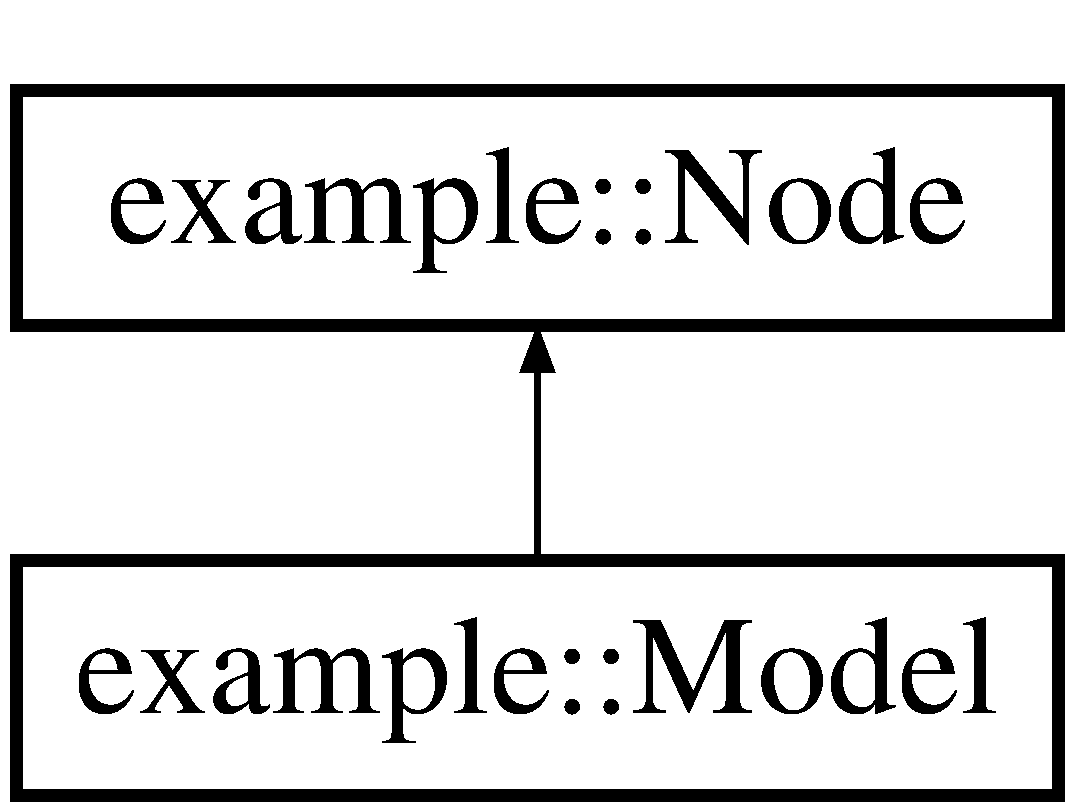
\includegraphics[height=2.000000cm]{classexample_1_1_model}
\end{center}
\end{figure}
\subsection*{Public Member Functions}
\begin{DoxyCompactItemize}
\item 
\mbox{\hyperlink{classexample_1_1_model_a0e1e9b91041e92ab9c45c5297a5c7a7a}{Model}} (char $\ast$path)
\item 
void \mbox{\hyperlink{classexample_1_1_model_ade64225bbb0381bbd5a8dddeac81d983}{render}} ()
\end{DoxyCompactItemize}


\subsection{Constructor \& Destructor Documentation}
\mbox{\Hypertarget{classexample_1_1_model_a0e1e9b91041e92ab9c45c5297a5c7a7a}\label{classexample_1_1_model_a0e1e9b91041e92ab9c45c5297a5c7a7a}} 
\index{example\+::\+Model@{example\+::\+Model}!Model@{Model}}
\index{Model@{Model}!example\+::\+Model@{example\+::\+Model}}
\subsubsection{\texorpdfstring{Model()}{Model()}}
{\footnotesize\ttfamily example\+::\+Model\+::\+Model (\begin{DoxyParamCaption}\item[{char $\ast$}]{path }\end{DoxyParamCaption})\hspace{0.3cm}{\ttfamily [inline]}}



\subsection{Member Function Documentation}
\mbox{\Hypertarget{classexample_1_1_model_ade64225bbb0381bbd5a8dddeac81d983}\label{classexample_1_1_model_ade64225bbb0381bbd5a8dddeac81d983}} 
\index{example\+::\+Model@{example\+::\+Model}!render@{render}}
\index{render@{render}!example\+::\+Model@{example\+::\+Model}}
\subsubsection{\texorpdfstring{render()}{render()}}
{\footnotesize\ttfamily void example\+::\+Model\+::render (\begin{DoxyParamCaption}{ }\end{DoxyParamCaption})\hspace{0.3cm}{\ttfamily [virtual]}}



Reimplemented from \mbox{\hyperlink{classexample_1_1_node_a6e9c30ac62693f7fa0a4080202df45df}{example\+::\+Node}}.



The documentation for this class was generated from the following files\+:\begin{DoxyCompactItemize}
\item 
D\+:/\+Git\+Kraken/3\+D\+Av\+\_\+2/src/\mbox{\hyperlink{_model_8hpp}{Model.\+hpp}}\item 
D\+:/\+Git\+Kraken/3\+D\+Av\+\_\+2/src/\mbox{\hyperlink{_model_8cpp}{Model.\+cpp}}\end{DoxyCompactItemize}

\hypertarget{classexample_1_1_node}{}\section{example\+:\+:Node Class Reference}
\label{classexample_1_1_node}\index{example\+::\+Node@{example\+::\+Node}}


{\ttfamily \#include $<$Node.\+hpp$>$}

Inheritance diagram for example\+:\+:Node\+:\begin{figure}[H]
\begin{center}
\leavevmode
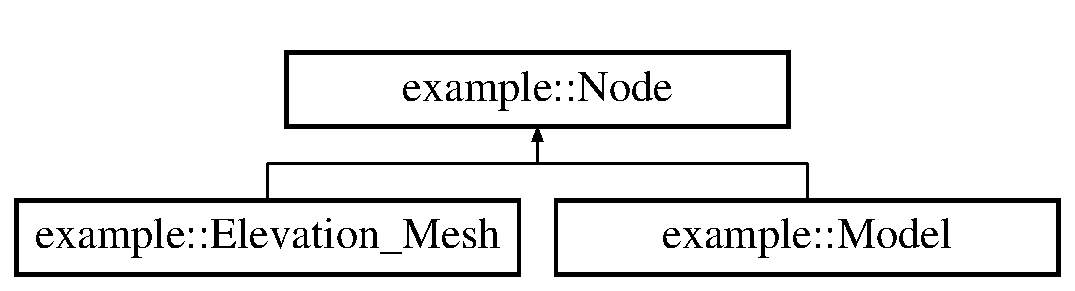
\includegraphics[height=2.000000cm]{classexample_1_1_node}
\end{center}
\end{figure}
\subsection*{Public Member Functions}
\begin{DoxyCompactItemize}
\item 
\mbox{\hyperlink{classexample_1_1_node_a27eff42d7d0078761627f2fa5ede06bc}{Node}} ()
\item 
virtual void \mbox{\hyperlink{classexample_1_1_node_a6e9c30ac62693f7fa0a4080202df45df}{render}} ()
\item 
virtual void \mbox{\hyperlink{classexample_1_1_node_a6d570b9e13063686b8057d8f561e196e}{update}} ()
\end{DoxyCompactItemize}


\subsection{Constructor \& Destructor Documentation}
\mbox{\Hypertarget{classexample_1_1_node_a27eff42d7d0078761627f2fa5ede06bc}\label{classexample_1_1_node_a27eff42d7d0078761627f2fa5ede06bc}} 
\index{example\+::\+Node@{example\+::\+Node}!Node@{Node}}
\index{Node@{Node}!example\+::\+Node@{example\+::\+Node}}
\subsubsection{\texorpdfstring{Node()}{Node()}}
{\footnotesize\ttfamily example\+::\+Node\+::\+Node (\begin{DoxyParamCaption}{ }\end{DoxyParamCaption})\hspace{0.3cm}{\ttfamily [inline]}}



\subsection{Member Function Documentation}
\mbox{\Hypertarget{classexample_1_1_node_a6e9c30ac62693f7fa0a4080202df45df}\label{classexample_1_1_node_a6e9c30ac62693f7fa0a4080202df45df}} 
\index{example\+::\+Node@{example\+::\+Node}!render@{render}}
\index{render@{render}!example\+::\+Node@{example\+::\+Node}}
\subsubsection{\texorpdfstring{render()}{render()}}
{\footnotesize\ttfamily virtual void example\+::\+Node\+::render (\begin{DoxyParamCaption}{ }\end{DoxyParamCaption})\hspace{0.3cm}{\ttfamily [inline]}, {\ttfamily [virtual]}}



Reimplemented in \mbox{\hyperlink{classexample_1_1_elevation___mesh_a67216abcf32e92e3da91810e10822c6e}{example\+::\+Elevation\+\_\+\+Mesh}}, and \mbox{\hyperlink{classexample_1_1_model_ade64225bbb0381bbd5a8dddeac81d983}{example\+::\+Model}}.

\mbox{\Hypertarget{classexample_1_1_node_a6d570b9e13063686b8057d8f561e196e}\label{classexample_1_1_node_a6d570b9e13063686b8057d8f561e196e}} 
\index{example\+::\+Node@{example\+::\+Node}!update@{update}}
\index{update@{update}!example\+::\+Node@{example\+::\+Node}}
\subsubsection{\texorpdfstring{update()}{update()}}
{\footnotesize\ttfamily virtual void example\+::\+Node\+::update (\begin{DoxyParamCaption}{ }\end{DoxyParamCaption})\hspace{0.3cm}{\ttfamily [inline]}, {\ttfamily [virtual]}}



The documentation for this class was generated from the following file\+:\begin{DoxyCompactItemize}
\item 
D\+:/\+Git\+Kraken/3\+D\+Av\+\_\+2/src/\mbox{\hyperlink{_node_8hpp}{Node.\+hpp}}\end{DoxyCompactItemize}

\hypertarget{classexample_1_1_scene}{}\section{example\+:\+:Scene Class Reference}
\label{classexample_1_1_scene}\index{example\+::\+Scene@{example\+::\+Scene}}


{\ttfamily \#include $<$Scene.\+hpp$>$}

\subsection*{Public Member Functions}
\begin{DoxyCompactItemize}
\item 
\mbox{\hyperlink{classexample_1_1_scene_a70c556631b334b52249e8c3de5dfbdb3}{Scene}} ()
\item 
void \mbox{\hyperlink{classexample_1_1_scene_ab11cb4f5a9023180eb1a9f5c9265f1ec}{add}} (shared\+\_\+ptr$<$ \mbox{\hyperlink{classexample_1_1_node}{Node}} $>$ node)
\item 
void \mbox{\hyperlink{classexample_1_1_scene_a6e8672b9fab7eaa38bc039467dc0b66a}{render}} ()
\end{DoxyCompactItemize}


\subsection{Constructor \& Destructor Documentation}
\mbox{\Hypertarget{classexample_1_1_scene_a70c556631b334b52249e8c3de5dfbdb3}\label{classexample_1_1_scene_a70c556631b334b52249e8c3de5dfbdb3}} 
\index{example\+::\+Scene@{example\+::\+Scene}!Scene@{Scene}}
\index{Scene@{Scene}!example\+::\+Scene@{example\+::\+Scene}}
\subsubsection{\texorpdfstring{Scene()}{Scene()}}
{\footnotesize\ttfamily example\+::\+Scene\+::\+Scene (\begin{DoxyParamCaption}{ }\end{DoxyParamCaption})\hspace{0.3cm}{\ttfamily [inline]}}



\subsection{Member Function Documentation}
\mbox{\Hypertarget{classexample_1_1_scene_ab11cb4f5a9023180eb1a9f5c9265f1ec}\label{classexample_1_1_scene_ab11cb4f5a9023180eb1a9f5c9265f1ec}} 
\index{example\+::\+Scene@{example\+::\+Scene}!add@{add}}
\index{add@{add}!example\+::\+Scene@{example\+::\+Scene}}
\subsubsection{\texorpdfstring{add()}{add()}}
{\footnotesize\ttfamily void example\+::\+Scene\+::add (\begin{DoxyParamCaption}\item[{shared\+\_\+ptr$<$ \mbox{\hyperlink{classexample_1_1_node}{Node}} $>$}]{node }\end{DoxyParamCaption})\hspace{0.3cm}{\ttfamily [inline]}}

\mbox{\Hypertarget{classexample_1_1_scene_a6e8672b9fab7eaa38bc039467dc0b66a}\label{classexample_1_1_scene_a6e8672b9fab7eaa38bc039467dc0b66a}} 
\index{example\+::\+Scene@{example\+::\+Scene}!render@{render}}
\index{render@{render}!example\+::\+Scene@{example\+::\+Scene}}
\subsubsection{\texorpdfstring{render()}{render()}}
{\footnotesize\ttfamily void example\+::\+Scene\+::render (\begin{DoxyParamCaption}{ }\end{DoxyParamCaption})\hspace{0.3cm}{\ttfamily [inline]}}



The documentation for this class was generated from the following file\+:\begin{DoxyCompactItemize}
\item 
D\+:/\+Git\+Kraken/3\+D\+Av\+\_\+2/src/\mbox{\hyperlink{_scene_8hpp}{Scene.\+hpp}}\end{DoxyCompactItemize}

\hypertarget{classexample_1_1_view}{}\section{example\+:\+:View Class Reference}
\label{classexample_1_1_view}\index{example\+::\+View@{example\+::\+View}}


{\ttfamily \#include $<$View.\+hpp$>$}

\subsection*{Public Member Functions}
\begin{DoxyCompactItemize}
\item 
\mbox{\hyperlink{classexample_1_1_view_ae7f67b78cdd174449edc93960f29d9f4}{View}} (int width, int height, shared\+\_\+ptr$<$ \mbox{\hyperlink{classexample_1_1_scene}{Scene}} $>$ scene)
\begin{DoxyCompactList}\small\item\em Creates a view with the specified dymensions And sets the scene which is going to be rendered. \end{DoxyCompactList}\item 
void \mbox{\hyperlink{classexample_1_1_view_ac0b18fc4d2abe1abca6940c55313ef3b}{update}} (\mbox{\hyperlink{classexample_1_1_input_af6bf4fd763ca01bd106ca3b03f162e3d}{Input\+::\+Input\+Data}} input\+\_\+data)
\begin{DoxyCompactList}\small\item\em Applies the imput data to the view Now it\textquotesingle{}s rotating and translating the view. \end{DoxyCompactList}\item 
void \mbox{\hyperlink{classexample_1_1_view_a10ea89fc705a2ba2252f673499524bf2}{render}} ()
\begin{DoxyCompactList}\small\item\em Renders every node in the scene. \end{DoxyCompactList}\item 
void \mbox{\hyperlink{classexample_1_1_view_a2396337a1db393acefb174e386cde7d1}{resize}} (int width, int height)
\begin{DoxyCompactList}\small\item\em Resizes the view given the window dimensions. \end{DoxyCompactList}\end{DoxyCompactItemize}


\subsection{Constructor \& Destructor Documentation}
\mbox{\Hypertarget{classexample_1_1_view_ae7f67b78cdd174449edc93960f29d9f4}\label{classexample_1_1_view_ae7f67b78cdd174449edc93960f29d9f4}} 
\index{example\+::\+View@{example\+::\+View}!View@{View}}
\index{View@{View}!example\+::\+View@{example\+::\+View}}
\subsubsection{\texorpdfstring{View()}{View()}}
{\footnotesize\ttfamily example\+::\+View\+::\+View (\begin{DoxyParamCaption}\item[{int}]{width,  }\item[{int}]{height,  }\item[{shared\+\_\+ptr$<$ \mbox{\hyperlink{classexample_1_1_scene}{Scene}} $>$}]{scene }\end{DoxyParamCaption})}



Creates a view with the specified dymensions And sets the scene which is going to be rendered. 



\subsection{Member Function Documentation}
\mbox{\Hypertarget{classexample_1_1_view_a10ea89fc705a2ba2252f673499524bf2}\label{classexample_1_1_view_a10ea89fc705a2ba2252f673499524bf2}} 
\index{example\+::\+View@{example\+::\+View}!render@{render}}
\index{render@{render}!example\+::\+View@{example\+::\+View}}
\subsubsection{\texorpdfstring{render()}{render()}}
{\footnotesize\ttfamily void example\+::\+View\+::render (\begin{DoxyParamCaption}{ }\end{DoxyParamCaption})}



Renders every node in the scene. 

\mbox{\Hypertarget{classexample_1_1_view_a2396337a1db393acefb174e386cde7d1}\label{classexample_1_1_view_a2396337a1db393acefb174e386cde7d1}} 
\index{example\+::\+View@{example\+::\+View}!resize@{resize}}
\index{resize@{resize}!example\+::\+View@{example\+::\+View}}
\subsubsection{\texorpdfstring{resize()}{resize()}}
{\footnotesize\ttfamily void example\+::\+View\+::resize (\begin{DoxyParamCaption}\item[{int}]{width,  }\item[{int}]{height }\end{DoxyParamCaption})}



Resizes the view given the window dimensions. 


\begin{DoxyParams}{Parameters}
{\em width} & window width \\
\hline
{\em width} & window height \\
\hline
\end{DoxyParams}
\mbox{\Hypertarget{classexample_1_1_view_ac0b18fc4d2abe1abca6940c55313ef3b}\label{classexample_1_1_view_ac0b18fc4d2abe1abca6940c55313ef3b}} 
\index{example\+::\+View@{example\+::\+View}!update@{update}}
\index{update@{update}!example\+::\+View@{example\+::\+View}}
\subsubsection{\texorpdfstring{update()}{update()}}
{\footnotesize\ttfamily void example\+::\+View\+::update (\begin{DoxyParamCaption}\item[{\mbox{\hyperlink{classexample_1_1_input_af6bf4fd763ca01bd106ca3b03f162e3d}{Input\+::\+Input\+Data}}}]{input\+\_\+data }\end{DoxyParamCaption})}



Applies the imput data to the view Now it\textquotesingle{}s rotating and translating the view. 



The documentation for this class was generated from the following files\+:\begin{DoxyCompactItemize}
\item 
D\+:/\+Git\+Kraken/3\+D\+Av\+\_\+2/src/\mbox{\hyperlink{_view_8hpp}{View.\+hpp}}\item 
D\+:/\+Git\+Kraken/3\+D\+Av\+\_\+2/src/\mbox{\hyperlink{_view_8cpp}{View.\+cpp}}\end{DoxyCompactItemize}

\chapter{File Documentation}
\hypertarget{_color___buffer_8hpp}{}\section{D\+:/\+Git\+Kraken/3\+D\+Av\+\_\+2/src/\+Color\+\_\+\+Buffer.hpp File Reference}
\label{_color___buffer_8hpp}\index{D\+:/\+Git\+Kraken/3\+D\+Av\+\_\+2/src/\+Color\+\_\+\+Buffer.\+hpp@{D\+:/\+Git\+Kraken/3\+D\+Av\+\_\+2/src/\+Color\+\_\+\+Buffer.\+hpp}}
\subsection*{Classes}
\begin{DoxyCompactItemize}
\item 
class \mbox{\hyperlink{classoglsl_1_1_color___buffer}{oglsl\+::\+Color\+\_\+\+Buffer}}
\end{DoxyCompactItemize}
\subsection*{Namespaces}
\begin{DoxyCompactItemize}
\item 
 \mbox{\hyperlink{namespaceoglsl}{oglsl}}
\end{DoxyCompactItemize}

\hypertarget{_color___buffer___rgba8888_8hpp}{}\section{D\+:/\+Git\+Kraken/3\+D\+Av\+\_\+2/src/\+Color\+\_\+\+Buffer\+\_\+\+Rgba8888.hpp File Reference}
\label{_color___buffer___rgba8888_8hpp}\index{D\+:/\+Git\+Kraken/3\+D\+Av\+\_\+2/src/\+Color\+\_\+\+Buffer\+\_\+\+Rgba8888.\+hpp@{D\+:/\+Git\+Kraken/3\+D\+Av\+\_\+2/src/\+Color\+\_\+\+Buffer\+\_\+\+Rgba8888.\+hpp}}
{\ttfamily \#include \char`\"{}Color\+\_\+\+Buffer.\+hpp\char`\"{}}\newline
{\ttfamily \#include $<$S\+F\+M\+L/\+Open\+G\+L.\+hpp$>$}\newline
{\ttfamily \#include $<$stdint.\+h$>$}\newline
{\ttfamily \#include $<$vector$>$}\newline
\subsection*{Classes}
\begin{DoxyCompactItemize}
\item 
class \mbox{\hyperlink{classexample_1_1_color___buffer___rgba8888}{example\+::\+Color\+\_\+\+Buffer\+\_\+\+Rgba8888}}
\item 
struct \mbox{\hyperlink{structexample_1_1_color___buffer___rgba8888_1_1_color}{example\+::\+Color\+\_\+\+Buffer\+\_\+\+Rgba8888\+::\+Color}}
\end{DoxyCompactItemize}
\subsection*{Namespaces}
\begin{DoxyCompactItemize}
\item 
 \mbox{\hyperlink{namespaceexample}{example}}
\end{DoxyCompactItemize}

\hypertarget{_cube_8cpp}{}\section{D\+:/\+Git\+Kraken/3\+D\+Av\+\_\+2/src/\+Cube.cpp File Reference}
\label{_cube_8cpp}\index{D\+:/\+Git\+Kraken/3\+D\+Av\+\_\+2/src/\+Cube.\+cpp@{D\+:/\+Git\+Kraken/3\+D\+Av\+\_\+2/src/\+Cube.\+cpp}}
{\ttfamily \#include $<$G\+L/glew.\+h$>$}\newline
{\ttfamily \#include \char`\"{}Cube.\+hpp\char`\"{}}\newline
{\ttfamily \#include $<$S\+F\+M\+L/\+Open\+G\+L.\+hpp$>$}\newline
\subsection*{Namespaces}
\begin{DoxyCompactItemize}
\item 
 \mbox{\hyperlink{namespaceexample}{example}}
\end{DoxyCompactItemize}

\hypertarget{_cube_8hpp}{}\section{D\+:/\+Git\+Kraken/3\+D\+Av\+\_\+2/src/\+Cube.hpp File Reference}
\label{_cube_8hpp}\index{D\+:/\+Git\+Kraken/3\+D\+Av\+\_\+2/src/\+Cube.\+hpp@{D\+:/\+Git\+Kraken/3\+D\+Av\+\_\+2/src/\+Cube.\+hpp}}
{\ttfamily \#include $<$S\+F\+M\+L/\+Open\+G\+L.\+hpp$>$}\newline
\subsection*{Classes}
\begin{DoxyCompactItemize}
\item 
class \mbox{\hyperlink{classexample_1_1_cube}{example\+::\+Cube}}
\end{DoxyCompactItemize}
\subsection*{Namespaces}
\begin{DoxyCompactItemize}
\item 
 \mbox{\hyperlink{namespaceexample}{example}}
\end{DoxyCompactItemize}

\hypertarget{_elevation___mesh_8cpp}{}\section{D\+:/\+Git\+Kraken/3\+D\+Av\+\_\+2/src/\+Elevation\+\_\+\+Mesh.cpp File Reference}
\label{_elevation___mesh_8cpp}\index{D\+:/\+Git\+Kraken/3\+D\+Av\+\_\+2/src/\+Elevation\+\_\+\+Mesh.\+cpp@{D\+:/\+Git\+Kraken/3\+D\+Av\+\_\+2/src/\+Elevation\+\_\+\+Mesh.\+cpp}}
{\ttfamily \#include $<$vector$>$}\newline
{\ttfamily \#include $<$G\+L/glew.\+h$>$}\newline
{\ttfamily \#include \char`\"{}Elevation\+\_\+\+Mesh.\+hpp\char`\"{}}\newline
{\ttfamily \#include $<$S\+F\+M\+L/\+Open\+G\+L.\+hpp$>$}\newline
{\ttfamily \#include \char`\"{}Color\+\_\+\+Buffer\+\_\+\+Rgba8888.\+hpp\char`\"{}}\newline
{\ttfamily \#include $<$targa.\+h$>$}\newline
\subsection*{Namespaces}
\begin{DoxyCompactItemize}
\item 
 \mbox{\hyperlink{namespaceexample}{example}}
\end{DoxyCompactItemize}

\hypertarget{_elevation___mesh_8hpp}{}\section{D\+:/\+Git\+Kraken/3\+D\+Av\+\_\+2/src/\+Elevation\+\_\+\+Mesh.hpp File Reference}
\label{_elevation___mesh_8hpp}\index{D\+:/\+Git\+Kraken/3\+D\+Av\+\_\+2/src/\+Elevation\+\_\+\+Mesh.\+hpp@{D\+:/\+Git\+Kraken/3\+D\+Av\+\_\+2/src/\+Elevation\+\_\+\+Mesh.\+hpp}}
{\ttfamily \#include $<$memory$>$}\newline
{\ttfamily \#include $<$S\+F\+M\+L/\+Open\+G\+L.\+hpp$>$}\newline
{\ttfamily \#include $<$glm/glm.\+hpp$>$}\newline
{\ttfamily \#include \char`\"{}Node.\+hpp\char`\"{}}\newline
{\ttfamily \#include \char`\"{}Shader\+\_\+\+Program.\+hpp\char`\"{}}\newline
\subsection*{Classes}
\begin{DoxyCompactItemize}
\item 
class \mbox{\hyperlink{classoglsl_1_1_elevation___mesh}{oglsl\+::\+Elevation\+\_\+\+Mesh}}
\end{DoxyCompactItemize}
\subsection*{Namespaces}
\begin{DoxyCompactItemize}
\item 
 \mbox{\hyperlink{namespaceoglsl}{oglsl}}
\end{DoxyCompactItemize}
\subsection*{Typedefs}
\begin{DoxyCompactItemize}
\item 
typedef Color\+\_\+\+Buffer\+\_\+\+Rgba8888 \mbox{\hyperlink{namespaceoglsl_a3f3bf2d9553fda1a155d7492ee30d7d0}{oglsl\+::\+Texture}}
\end{DoxyCompactItemize}

\hypertarget{_input_8hpp}{}\section{D\+:/\+Git\+Kraken/3\+D\+Av\+\_\+2/src/\+Input.hpp File Reference}
\label{_input_8hpp}\index{D\+:/\+Git\+Kraken/3\+D\+Av\+\_\+2/src/\+Input.\+hpp@{D\+:/\+Git\+Kraken/3\+D\+Av\+\_\+2/src/\+Input.\+hpp}}
{\ttfamily \#include $<$map$>$}\newline
{\ttfamily \#include $<$memory$>$}\newline
{\ttfamily \#include \char`\"{}Variant.\+hpp\char`\"{}}\newline
{\ttfamily \#include $<$S\+F\+M\+L/\+Window.\+hpp$>$}\newline
{\ttfamily \#include $<$S\+F\+M\+L/\+Open\+G\+L.\+hpp$>$}\newline
{\ttfamily \#include $<$glm/glm.\+hpp$>$}\newline
\subsection*{Classes}
\begin{DoxyCompactItemize}
\item 
class \mbox{\hyperlink{classoglsl_1_1_input}{oglsl\+::\+Input}}
\begin{DoxyCompactList}\small\item\em Controls user input. \end{DoxyCompactList}\end{DoxyCompactItemize}
\subsection*{Namespaces}
\begin{DoxyCompactItemize}
\item 
 \mbox{\hyperlink{namespaceoglsl}{oglsl}}
\end{DoxyCompactItemize}

\hypertarget{main_8cpp}{}\section{D\+:/\+Git\+Kraken/3\+D\+Av\+\_\+2/src/main.cpp File Reference}
\label{main_8cpp}\index{D\+:/\+Git\+Kraken/3\+D\+Av\+\_\+2/src/main.\+cpp@{D\+:/\+Git\+Kraken/3\+D\+Av\+\_\+2/src/main.\+cpp}}
{\ttfamily \#include $<$cassert$>$}\newline
{\ttfamily \#include $<$string$>$}\newline
{\ttfamily \#include \char`\"{}my\+Scene.\+hpp\char`\"{}}\newline
{\ttfamily \#include \char`\"{}View.\+hpp\char`\"{}}\newline
{\ttfamily \#include $<$S\+F\+M\+L/\+Window.\+hpp$>$}\newline
{\ttfamily \#include $<$S\+F\+M\+L/\+Open\+G\+L.\+hpp$>$}\newline
{\ttfamily \#include \char`\"{}Input.\+hpp\char`\"{}}\newline
\subsection*{Functions}
\begin{DoxyCompactItemize}
\item 
int \mbox{\hyperlink{main_8cpp_ae66f6b31b5ad750f1fe042a706a4e3d4}{main}} ()
\end{DoxyCompactItemize}


\subsection{Function Documentation}
\mbox{\Hypertarget{main_8cpp_ae66f6b31b5ad750f1fe042a706a4e3d4}\label{main_8cpp_ae66f6b31b5ad750f1fe042a706a4e3d4}} 
\index{main.\+cpp@{main.\+cpp}!main@{main}}
\index{main@{main}!main.\+cpp@{main.\+cpp}}
\subsubsection{\texorpdfstring{main()}{main()}}
{\footnotesize\ttfamily int main (\begin{DoxyParamCaption}{ }\end{DoxyParamCaption})}


\hypertarget{_mesh_8cpp}{}\section{D\+:/\+Git\+Kraken/3\+D\+Av\+\_\+2/src/\+Mesh.cpp File Reference}
\label{_mesh_8cpp}\index{D\+:/\+Git\+Kraken/3\+D\+Av\+\_\+2/src/\+Mesh.\+cpp@{D\+:/\+Git\+Kraken/3\+D\+Av\+\_\+2/src/\+Mesh.\+cpp}}
{\ttfamily \#include \char`\"{}Mesh.\+hpp\char`\"{}}\newline
\subsection*{Namespaces}
\begin{DoxyCompactItemize}
\item 
 \mbox{\hyperlink{namespaceoglsl}{oglsl}}
\end{DoxyCompactItemize}

\hypertarget{_mesh_8hpp}{}\section{D\+:/\+Git\+Kraken/3\+D\+Av\+\_\+2/src/\+Mesh.hpp File Reference}
\label{_mesh_8hpp}\index{D\+:/\+Git\+Kraken/3\+D\+Av\+\_\+2/src/\+Mesh.\+hpp@{D\+:/\+Git\+Kraken/3\+D\+Av\+\_\+2/src/\+Mesh.\+hpp}}
{\ttfamily \#include $<$memory$>$}\newline
{\ttfamily \#include $<$string$>$}\newline
{\ttfamily \#include $<$vector$>$}\newline
{\ttfamily \#include $<$glm/glm.\+hpp$>$}\newline
{\ttfamily \#include $<$glm/gtc/matrix\+\_\+transform.\+hpp$>$}\newline
{\ttfamily \#include $<$glm/gtc/type\+\_\+ptr.\+hpp$>$}\newline
{\ttfamily \#include $<$G\+L/glew.\+h$>$}\newline
{\ttfamily \#include $<$S\+F\+M\+L/\+Open\+G\+L.\+hpp$>$}\newline
{\ttfamily \#include \char`\"{}Color\+\_\+\+Buffer\+\_\+\+Rgba8888.\+hpp\char`\"{}}\newline
{\ttfamily \#include \char`\"{}Shader\+\_\+\+Program.\+hpp\char`\"{}}\newline
\subsection*{Classes}
\begin{DoxyCompactItemize}
\item 
class \mbox{\hyperlink{classoglsl_1_1_mesh}{oglsl\+::\+Mesh}}
\begin{DoxyCompactList}\small\item\em Represents the mesh data of the models. \end{DoxyCompactList}\end{DoxyCompactItemize}
\subsection*{Namespaces}
\begin{DoxyCompactItemize}
\item 
 \mbox{\hyperlink{namespaceoglsl}{oglsl}}
\end{DoxyCompactItemize}

\hypertarget{_model_8cpp}{}\section{D\+:/\+Git\+Kraken/3\+D\+Av\+\_\+2/src/\+Model.cpp File Reference}
\label{_model_8cpp}\index{D\+:/\+Git\+Kraken/3\+D\+Av\+\_\+2/src/\+Model.\+cpp@{D\+:/\+Git\+Kraken/3\+D\+Av\+\_\+2/src/\+Model.\+cpp}}
{\ttfamily \#include \char`\"{}Model.\+hpp\char`\"{}}\newline
{\ttfamily \#include $<$targa.\+h$>$}\newline
\subsection*{Namespaces}
\begin{DoxyCompactItemize}
\item 
 \mbox{\hyperlink{namespaceoglsl}{oglsl}}
\end{DoxyCompactItemize}

\hypertarget{_model_8hpp}{}\section{D\+:/\+Git\+Kraken/3\+D\+Av\+\_\+2/src/\+Model.hpp File Reference}
\label{_model_8hpp}\index{D\+:/\+Git\+Kraken/3\+D\+Av\+\_\+2/src/\+Model.\+hpp@{D\+:/\+Git\+Kraken/3\+D\+Av\+\_\+2/src/\+Model.\+hpp}}
{\ttfamily \#include $<$iostream$>$}\newline
{\ttfamily \#include $<$scene.\+h$>$}\newline
{\ttfamily \#include $<$Importer.\+hpp$>$}\newline
{\ttfamily \#include $<$postprocess.\+h$>$}\newline
{\ttfamily \#include \char`\"{}Node.\+hpp\char`\"{}}\newline
{\ttfamily \#include \char`\"{}Mesh.\+hpp\char`\"{}}\newline
\subsection*{Classes}
\begin{DoxyCompactItemize}
\item 
class \mbox{\hyperlink{classexample_1_1_model}{example\+::\+Model}}
\end{DoxyCompactItemize}
\subsection*{Namespaces}
\begin{DoxyCompactItemize}
\item 
 \mbox{\hyperlink{namespaceexample}{example}}
\end{DoxyCompactItemize}

\hypertarget{_node_8hpp}{}\section{D\+:/\+Git\+Kraken/3\+D\+Av\+\_\+2/src/\+Node.hpp File Reference}
\label{_node_8hpp}\index{D\+:/\+Git\+Kraken/3\+D\+Av\+\_\+2/src/\+Node.\+hpp@{D\+:/\+Git\+Kraken/3\+D\+Av\+\_\+2/src/\+Node.\+hpp}}
\subsection*{Classes}
\begin{DoxyCompactItemize}
\item 
class \mbox{\hyperlink{classexample_1_1_node}{example\+::\+Node}}
\end{DoxyCompactItemize}
\subsection*{Namespaces}
\begin{DoxyCompactItemize}
\item 
 \mbox{\hyperlink{namespaceexample}{example}}
\end{DoxyCompactItemize}

\hypertarget{_scene_8hpp}{}\section{D\+:/\+Git\+Kraken/3\+D\+Av\+\_\+2/src/\+Scene.hpp File Reference}
\label{_scene_8hpp}\index{D\+:/\+Git\+Kraken/3\+D\+Av\+\_\+2/src/\+Scene.\+hpp@{D\+:/\+Git\+Kraken/3\+D\+Av\+\_\+2/src/\+Scene.\+hpp}}
{\ttfamily \#include $<$map$>$}\newline
{\ttfamily \#include $<$memory$>$}\newline
{\ttfamily \#include $<$vector$>$}\newline
{\ttfamily \#include \char`\"{}Node.\+hpp\char`\"{}}\newline
{\ttfamily \#include \char`\"{}Camera.\+hpp\char`\"{}}\newline
{\ttfamily \#include \char`\"{}Skybox.\+hpp\char`\"{}}\newline
{\ttfamily \#include \char`\"{}Shader\+\_\+\+Program.\+hpp\char`\"{}}\newline
{\ttfamily \#include \char`\"{}Vertex\+\_\+\+Shader.\+hpp\char`\"{}}\newline
{\ttfamily \#include \char`\"{}Fragment\+\_\+\+Shader.\+hpp\char`\"{}}\newline
{\ttfamily \#include \char`\"{}Input.\+hpp\char`\"{}}\newline
\subsection*{Classes}
\begin{DoxyCompactItemize}
\item 
class \mbox{\hyperlink{classoglsl_1_1_scene}{oglsl\+::\+Scene}}
\end{DoxyCompactItemize}
\subsection*{Namespaces}
\begin{DoxyCompactItemize}
\item 
 \mbox{\hyperlink{namespaceoglsl}{oglsl}}
\end{DoxyCompactItemize}

\hypertarget{_view_8cpp}{}\section{D\+:/\+Git\+Kraken/3\+D\+Av\+\_\+2/src/\+View.cpp File Reference}
\label{_view_8cpp}\index{D\+:/\+Git\+Kraken/3\+D\+Av\+\_\+2/src/\+View.\+cpp@{D\+:/\+Git\+Kraken/3\+D\+Av\+\_\+2/src/\+View.\+cpp}}
{\ttfamily \#include \char`\"{}View.\+hpp\char`\"{}}\newline
{\ttfamily \#include $<$iostream$>$}\newline
{\ttfamily \#include $<$cassert$>$}\newline
{\ttfamily \#include $<$glm/glm.\+hpp$>$}\newline
{\ttfamily \#include $<$glm/gtc/matrix\+\_\+transform.\+hpp$>$}\newline
{\ttfamily \#include $<$glm/gtc/type\+\_\+ptr.\+hpp$>$}\newline
\subsection*{Namespaces}
\begin{DoxyCompactItemize}
\item 
 \mbox{\hyperlink{namespaceexample}{example}}
\end{DoxyCompactItemize}

\hypertarget{_view_8hpp}{}\section{D\+:/\+Git\+Kraken/3\+D\+Av\+\_\+2/src/\+View.hpp File Reference}
\label{_view_8hpp}\index{D\+:/\+Git\+Kraken/3\+D\+Av\+\_\+2/src/\+View.\+hpp@{D\+:/\+Git\+Kraken/3\+D\+Av\+\_\+2/src/\+View.\+hpp}}
{\ttfamily \#include $<$string$>$}\newline
{\ttfamily \#include $<$G\+L/glew.\+h$>$}\newline
{\ttfamily \#include \char`\"{}Cube.\+hpp\char`\"{}}\newline
{\ttfamily \#include \char`\"{}Scene.\+hpp\char`\"{}}\newline
{\ttfamily \#include \char`\"{}Input.\+hpp\char`\"{}}\newline
\subsection*{Classes}
\begin{DoxyCompactItemize}
\item 
class \mbox{\hyperlink{classoglsl_1_1_view}{oglsl\+::\+View}}
\begin{DoxyCompactList}\small\item\em D\+E\+P\+R\+E\+C\+A\+T\+ED. \end{DoxyCompactList}\end{DoxyCompactItemize}
\subsection*{Namespaces}
\begin{DoxyCompactItemize}
\item 
 \mbox{\hyperlink{namespaceoglsl}{oglsl}}
\end{DoxyCompactItemize}

%--- End generated contents ---

% Index
\backmatter
\newpage
\phantomsection
\clearemptydoublepage
\addcontentsline{toc}{chapter}{Index}
\printindex

\end{document}
